\documentclass[10,a4paperpaper,]{article}

  \title{Replication Report Rhemtulla et al 2012}
  \author{Anna Lohmann\textsuperscript{1}, \and Arjan Huizing
\textsuperscript{2}}
  \date{%
		\textsuperscript{1} Leiden University Medical Center\\%
		\textsuperscript{2} TNO (Netherlands Organization for Applied
Scientific Research)~\\[2ex]
		\today
   }
  


\newcommand{\iblue}{008080}
\newcommand{\igray}{d4dbde}

\newlength{\cslhangindent}
\setlength{\cslhangindent}{1.5em}
\newenvironment{CSLReferences}%
  {}%
  {\par}

% Author: Karol KozioL
% License: GPL-3
% Modified by: Sarah Wagner & Anna Lohmann

% % % packages -----------------------------------------------------------------------------------
\usepackage{amsmath}
\usepackage{array}
\usepackage{booktabs}
\usepackage{calc}
\usepackage{eso-pic}
\usepackage{fancyhdr}
\usepackage{fontspec}
\usepackage[left = 2.5cm, right = 2.5cm, top = 1.2cm, bottom = 1.2cm, includeheadfoot]{geometry}
\usepackage{graphicx}
\usepackage[utf8]{inputenc}
\usepackage{lastpage}
\usepackage{multirow}
\usepackage{tabularx} 
\usepackage{tikz}
\usepackage{titlesec}
\usepackage{xcolor, colortbl}
\usepackage{url} 
\usepackage[hidelinks]{hyperref} 
\usepackage{pmboxdraw}
\usepackage{placeins}
\usepackage{enumitem}
\usepackage{longtable}
\usepackage{lscape}
%\usepackage{verbatim}
%\makeatletter
%\def\verbatim@font{\scriptsize\ttfamily}
%\makeatother
%\RequirePackage[normalem]{ulem} %DIF PREAMBLE
%\RequirePackage{color}
%\providecommand{\tightlist}{%
%	\setlength{\itemsep}{0pt}\setlength{\parskip{0pt}}
\providecommand{\tightlist}{%
  \setlength{\itemsep}{0pt}\setlength{\parskip}{0pt}}
% % % settings -----------------------------------------------------------------------------------

% % custom colors
\definecolor{iblue}{HTML}{\iblue}
\definecolor{igray}{HTML}{\igray}

% definition of pagename
\newcommand\pagename{Page}

% % fonts 
\defaultfontfeatures{Mapping = tex-text}
\setmainfont[BoldFont = Lato-Bold.ttf, ItalicFont = Lato-Italic.ttf, BoldItalicFont = Lato-BoldItalic.ttf]{Lato-Regular.ttf}
\newfontfamily\headingfont[ItalicFont = Lato-BlackItalic.ttf]{Lato-Black.ttf}
%\setmonofont{Ubuntu Mono}
\setmonofont[Scale=0.90,
BoldFont=UbuntuMono-Bold.ttf,
%ItalicFont=UbuntuMono-Italic.ttf,
BoldItalicFont=UbuntuMono-BoldItalic.ttf
]{UbuntuMono-Regular.ttf}

\makeatletter
\def\verbatim@font{\linespread{1}\normalfont\ttfamily}
\makeatother

% % sections
\titleformat{\section}{\color{iblue}\headingfont\Large\bfseries}{\thesection}{1em}{}[\titlerule]
\titleformat{\subsection}{\color{iblue}\headingfont\large\bfseries}{\thesubsection}{1em}{}
\titleformat{\subsubsection}{\color{iblue}\headingfont\bfseries}{\thesubsubsection}{1em}{}

% % misc
\setlength{\parindent}{0em} 
\linespread{1.5}
\raggedright
\newcolumntype{C}{>{\centering\arraybackslash}X}


\makeatletter

% pagestyle titlepage
\fancypagestyle{customtitle}{
	\lhead{}
	\chead{}
	\rhead{}
	\makeatother
	\lfoot{}
	\cfoot{}
	\rfoot{}
}




% % % header and footer ---------------------------------------------------------------------------
\pagestyle{fancy}
\lhead{}
\chead{}
\rhead{}
\makeatother
\newlength{\myheight}
\lfoot{}
\cfoot{}
\rfoot{\pagename~\thepage \hspace{1pt} / \pageref{LastPage}}
\renewcommand\headrulewidth{0pt}
\renewcommand\footrulewidth{0pt}





\begin{document}


\renewcommand{\contentsname}{Table of Contents}

\renewcommand{\pagename}{Page}


\urlstyle{same}

\maketitle

\subsection*{Abstract}

This documents the replication attempt of the simulation study reported
in Rhemtulla, M., Brosseau-Liard, P. É., \& Savalei, V. (2012). When can
categorical variables be treated as continuous? A comparison of robust
continuous and categorical SEM estimation methods under suboptimal
conditions. \emph{Psychological Methods}, 17(3), 354--373.
\url{https://doi.org/10.1037/a0029315}. The study compared two different
estimation methods (robust Maximum Likelihood (ML) and categorical least
squares (cat-LS/ULSMV)) for fitting confirmatory factor analysis models
in the context of categorical variables. Our replication involved
writing simulation code based on the information provided in the
manuscript and the corresponding supplemental material. Information
provided in the original study was detailed and well structured, thus
allowing us to reimplement the study to the best of our knowledge.
Detailed result tables provided in the supplemental material allowed us
to compare our replicated results to the original results. \vskip 2em

\noindent\makebox[\textwidth]{\large Correspondence concerning this replication report should be addressed to:}

\par

\noindent\makebox[\textwidth]{\large a.l.lohmann@lumc.nl}

\par

\clearpage

\section{Introduction}

This replication report documents the replication attempt of the
simulation study:

Rhemtulla, M., Brosseau-Liard, P. É., \& Savalei, V. (2012). When can
categorical variables be treated as continuous? A comparison of robust
continuous and categorical SEM estimation methods under suboptimal
conditions. \emph{Psychological Methods}, 17(3), 354--373.
\url{https://doi.org/10.1037/a0029315}

Following the definition of Rougier et al. (2017) we understand the
replication of a published study as writing and running new code based
on the description provided in the original publication with the aim of
obtaining the same results.

\section{Method}

\subsection{Information basis}

The replication attempt was based on the information provided in the
original manuscript as well as the supplemental material accompanying
the publication. The main text provided a link to the supplements
(\url{http://dx.doi.org/10.1037/a0029315.supp}) which referred to the
website of the publisher where an additional pdf document with extensive
result tables was freely available.

\subsection{Data Generating Mechanism}

The information provided indicated that the following simulation factors
were systematically varied in a full-factorial design for generating the
artificial data.

\begin{longtable}[]{@{}
  >{\raggedright\arraybackslash}p{(\columnwidth - 4\tabcolsep) * \real{0.4000}}
  >{\raggedright\arraybackslash}p{(\columnwidth - 4\tabcolsep) * \real{0.1333}}
  >{\raggedright\arraybackslash}p{(\columnwidth - 4\tabcolsep) * \real{0.4667}}@{}}
\toprule
\begin{minipage}[b]{\linewidth}\raggedright
Simulation factor
\end{minipage} & \begin{minipage}[b]{\linewidth}\raggedright
No.~levels
\end{minipage} & \begin{minipage}[b]{\linewidth}\raggedright
Levels
\end{minipage} \\
\midrule
\endhead
\emph{Varied} & & \\
CFA model size & 2 & 10 indicators, 20 indicators \\
Underlying distribution & 2 & normal, non-normal \\
Number of categories & 6 & 2,3,4,5,6,7 \\
Threshold symmetry & 5 & symmetry, moderate asymmetry, moderate
asymmetry alternative, extreme asymmetry \\
Sample Size & 4 & 100, 150, 350, 600 \\
\emph{Fixed} & & \\
factor loadings & & 0.3, 0.4, 0.5, 0.6, 0.7 \\
factor correlation & & 0.3 \\
\bottomrule
\end{longtable}

This results in a total of 480 scenarios under which data is generated.
Each of these conditions was simulated with 1000 repetitions.

Generating data consisted of two steps. (1) Data was generated based on
the underlying distribution, CFA model and sample size. (2) The
generated data was categorized based on the given category thresholds
corresponding to a given number of categories and threshold symmetry.

\subsubsection{CFA model}

The CFA models underlying data generation were described as
\emph{``Model 1 was a two-factor CFA model with five indicators per
factor, for a total of 10 indicators. Factor loadings for the five
indicators were .3, .4, .5, .6, .7. {[}\ldots{]} The model was
identified by fixing the variances of each latent variable to 1.
Generated continuous variables had unit variance (prior to
categorization). Model 2 was identical to Model 1, but with 10
indicators per factor.''} (p.~359)

We translated this information into the following matrices: \[
\Lambda = 
  \left[ {\begin{array}{cc}
    0.3 & 0 \\
    0.4 & 0\\
    0.5 & 0\\
    0.6 & 0\\
    0.7 & 0\\
    0 & 0.3\\
    0 & 0.4\\
    0 & 0.5\\
    0 & 0.6\\
    0 & 0.7\\
  \end{array} } \right]\]

\[ 
\Psi = 
  \left[ {\begin{array}{cc}
    1 & 0.3 \\
    0.3 & 1\\
  \end{array} } \right]
\]

\[ 
\Theta = 
  \left[ {\begin{array}{cccccccccc}
    1 & 0 & 0 & 0 & 0 & 0 & 0 & 0 & 0 & 0 \\
    0 & 1 & 0 & 0 & 0 & 0 & 0 & 0 & 0 & 0\\
    0 & 0 & 1 & 0 & 0 & 0 & 0 & 0 & 0 & 0 \\
    0 & 0 & 0 & 1 & 0 & 0 & 0 & 0 & 0 & 0\\
    0 & 0 & 0 & 0 & 1 & 0 & 0 & 0 & 0 & 0 \\
    0 & 0 & 0 & 0 & 0 & 1 & 0 & 0 & 0 & 0\\
    0 & 0 & 0 & 0 & 0 & 0 & 1 & 0 & 0 & 0 \\
    0 & 0 & 0 & 0 & 0 & 0 & 0 & 1 & 0 & 0\\
    0 & 0 & 0 & 0 & 0 & 0 & 0 & 0 & 1 & 0 \\
    0 & 0 & 0 & 0 & 0 & 0 & 0 & 0 & 0 & 1\\
  \end{array} } \right]
\]

We used these matrices as input for the \texttt{model()} function of the
\texttt{simsem} package.

\subsubsection{Underlying distribution, CFA model size and Sample Size}

The original study indicated that data were generated using the
Fleishman (1978) and Vale Maurelli (1983) method. We emulated this
approach using the \texttt{generate()} function from the \texttt{simsem}
package (Version 0.5-16) with the parameter \texttt{inDist} set to
\texttt{NULL} in the normal case and to
\texttt{simsem::bindDist(skewness\ =\ 2,\ kurtosis\ =\ 7)} in the
non-normal case. The \texttt{model} parameter from the
\texttt{generate()} function was specified as detailed above. This
constituted the first step of the data generation.

\subsubsection{Number of categories and Threshold symmetry}

After data was generated based on the given CFA model and the underlying
distribution the resulting data was categorized into the number of
categories for the scenario at hand. For each number of categories and
each threshold symmetry, Z-scores for category thresholds could be
obtained from the first table of the supplemental material. The sample
covariance matrix of the resulting categorized data was tested for
positive definiteness. In case it was found to be non-positive definite
data was resampled with a different seed until it was positive definite.
Additionally, it was ensured that none of the generated variables had
zero variance. These measures are not documented in the original study
but were implemented to avoid errors in code execution. Hence, we do not
know whether or at which point in the simulation pipeline these issues
were dealt with in the original study.

\FloatBarrier 

\subsection{Investigated Methods}

The study compares the performance of robust normal theory maximum
likelihood (ML) and robust categorical least squares (ULS) methodology
for estimating confirmatory factor analysis (CFA) with ordinary
variables. The underlying CFA model was fit using each of the two
methods under investigation. The ULS estimator is referred to as both
cat-LS as well as ULS in the original study. We will refer to it as ULS
for consistency in this report.

\subsubsection{Robust normal theory maximum likelihood (ML)}

CFA's were carried out using the \texttt{cfa()} function of the
\texttt{lavaan} package (Version 0.6-11). For the \emph{Robust normal
theory maximum likelihood} approach we set the \texttt{estimator}
argument to \texttt{"MLVM"}.

\subsubsection{Robust categorical least squares (ULS)}

The \emph{Robust categorical least squares (ULS)} approach was also
implemented using the \texttt{cfa()} function from the \texttt{lavaan}
package . In this case the \texttt{estimator} argument was set to
\texttt{"ULSMV"}. Additionally, the \texttt{ordered} argument was set to
\texttt{TRUE}.

\subsection{Performance measures}

The models estimated using the two methods described above were compared
on various performance measures.

\subsubsection{Convergence Failures}

The original article assessed the number of convergence failures. We
implemented convergence failure via the \texttt{lavInspect()} function
with the \texttt{what} argument set to \texttt{"converged"}.

\subsubsection{Improper solutions}

The original study reports assessing the number of improper solutions.
The paper defines improper solution as \emph{``when cat-LS estimation
produced a factor loading greater than 1 or continuous ML estimation
produced a standardized factor loading greater than 1''} (p.~361) We
implemented convergence failure via the \texttt{lavInspect()} function
with the \texttt{what} argument set to \texttt{"post.check"}.

\subsubsection{Parameter Estimates}

We extracted parameter estimates from the fitted lavaan object using the
\texttt{lavInspect()} function.

\subsubsection{Parameter Bias}

The parameter bias was calculated as the difference of the mean estimate
per scenario and the true value \(\bar{\theta}-\theta\).

\subsubsection{Coverage}

For each iteration of each scenario it was assessed whether the
estimated parameter fell within 1.96 standard errors of the true value.
We used robust standard errors from the estimated model for this
assessment.

\subsection{Power}

In addition to the above mentioned analyses the study included a brief
evaluation of the relative power of the ML-based and the ULS-based
robust test statistics to detect a least major model misspecification.
For this purpose the authors fit a \emph{``one-factor model to the data
generated by Model 1 (the 10-indicator, two factor model) for the subset
of conditions in which the underlying distribution was normal and
thresholds were symmetrically distributed.''} (p.~369). This subset
corresponds to 60 of the 480 scenarios. We interpreted the above to
indicate that the same generated data as for the rest of the simulation
study was used. We hence filtered the generated data sets to only retain
the scenarios including model 1, normally distributed variables and
symmetrically distributed thresholds for categorization and fit a
one-factor model to each of the data sets that fit these criteria.

A p-value \textless{} 0.05 of the robust \(\chi^2\) statistic was used
to indicate a model misspecification.

\subsection{Technical implementation}

The original simulation study was carried out in EQS (Version 6.1) as
well as Mplus (Version 6.11). The authors of the original study report
that data generation was carried out in EQS and data analysis was
conducted using both EQS as well as Mplus. However, only results from
the Mplus analysis are reported. Our replication was implemented using
the R programming environment (details regarding software versions can
be obtained from the section Reproducibility Information). The
corresponding R code can be obtained from
\url{https://github.com/replisims/rhemtulla-2012}.

\subsection{Replicator degrees of freedom}

The following table provides an overview of replicator degrees of
freedom, i.e.~decisions that had to be made by the replicators because
of insufficient or contradicting information. Issues were resolved by
discussion among the replicators.

\begin{longtable}[]{@{}
  >{\raggedright\arraybackslash}p{(\columnwidth - 4\tabcolsep) * \real{0.3636}}
  >{\raggedright\arraybackslash}p{(\columnwidth - 4\tabcolsep) * \real{0.3636}}
  >{\raggedright\arraybackslash}p{(\columnwidth - 4\tabcolsep) * \real{0.2727}}@{}}
\toprule
\begin{minipage}[b]{\linewidth}\raggedright
Issue
\end{minipage} & \begin{minipage}[b]{\linewidth}\raggedright
Replicator decision
\end{minipage} & \begin{minipage}[b]{\linewidth}\raggedright
Justification
\end{minipage} \\
\midrule
\endhead
Data basis fig 1\&2, tab 1 & Simulate just one variable & It seemed
unlikely that dozens of variables from the models were collapsed \\
Factor loadings of Model 2 & Each factor loading is assumed to occur
twice & Both replicators assumed this to be most likely \\
Error handling & Case-wise deletion & Text indicated that ``cases'' were
removed \\
Number of scenarios & 480 & We assumed the ``420 conditions'' (p.~362)
was a typo as a full-factorial combination results in 480 scenarios
which was also mentioned on page 359. \\
\bottomrule
\end{longtable}

\subsubsection{Data basis for Figures 1 and 2}

The text indicated that the data underlying Figures 1 and 2 as well as
Table 1 were generated for each ``scenario'' and a sample size of
1,000,000. We interpreted this to mean that one variable of length
1,000,000 was generated according to the specifications of each scenario
although each scenario technically generated data according to an entire
CFA model.

\subsubsection{Factor loadings of model 2}

The original article indicated that \emph{``Model 2 was identical to
Model 1, but with 10 indicators per factor.''}(p.~359) No additional
information regarding the factor loadings for these additional factor
loadings was provided. We hence assumed that additional indicators
reused the same set of factor loadings such that each loading occurred
twice.

\subsubsection{Error handling}

The original study describes three types of errors: Failures of
convergence, negative variance (i.e.~`Heywood' cases), and outliers
which they define as cases with a standard error greater than 1. The
authors mention nearly all of the errors they encountered occured under
small sample sizes (\emph{N} = 100 or 150). Furthermore, the supplied
supplemental contains tables detailing exactly how many errors were
found and under which conditions they occurred. The authors describe
excluding cases where errors occurred from further analysis. It is
however not clear if this exclusion was done for the estimation method
under which it occurred (case-wise deletion), or for both the ML and ULS
estimation methods (list-wise deletion). We considered case-wise more
likely, as the language used in the article seems to imply that a case
corresponds to a single method. Additionally, a list-wise approach would
be more wasteful.

\subsubsection{Number of scenarios}

Contrary to the 480 scenarios described in the methods section, the
result section mentions 420 conditions (p.~362). As 480 is consistent
with the number of scenarios obtained by fully crossing all simulation
factors described, we assumed the 420 to be a typo.

\section{Results}

\subsection{Replication of result figures}

The original study provides descriptives for the simulated data in two
figures. Figure 1 and Figure 2 of the original manuscript

\subsubsection{Figure 3 and 4 Parameter estimates (factor loadings)}

\begin{figure}
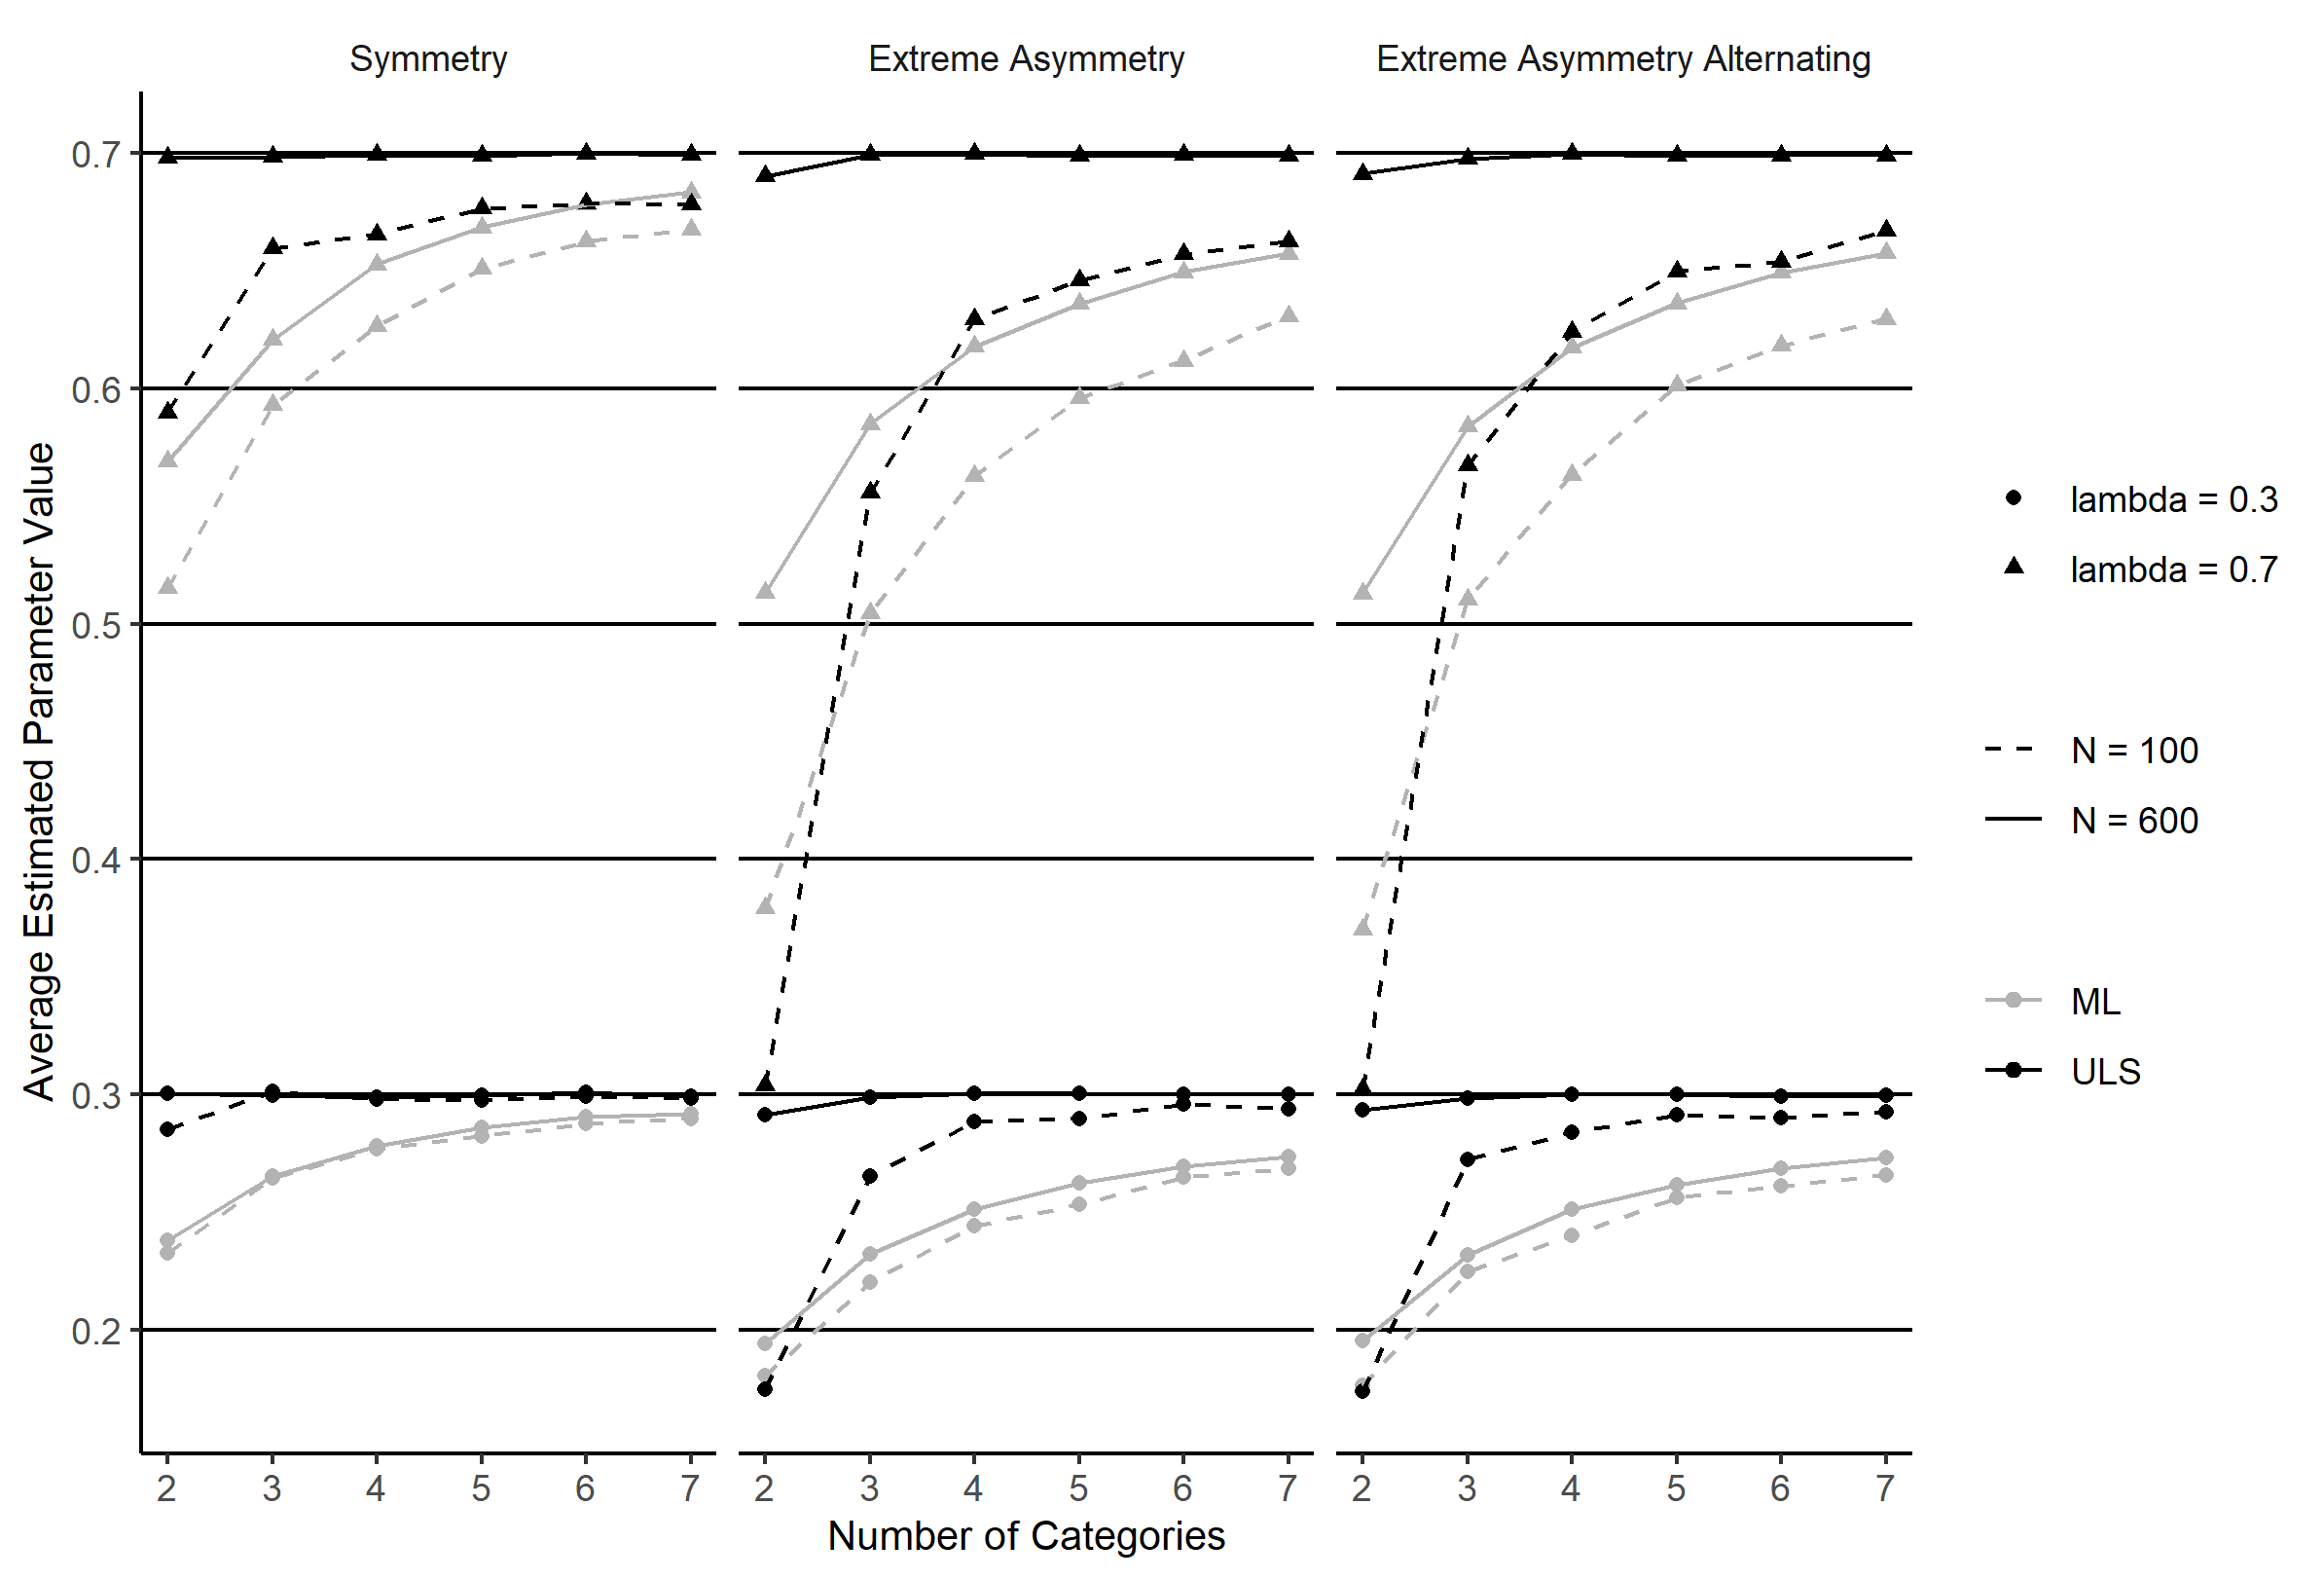
\includegraphics[width=0.49\linewidth]{./figures/fig_3} 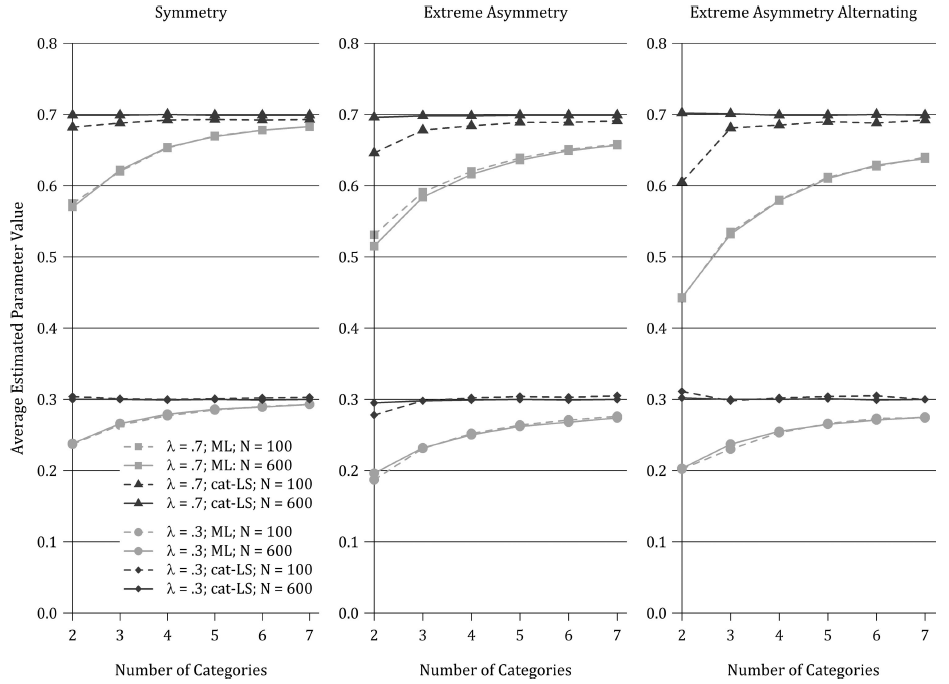
\includegraphics[width=0.49\linewidth]{./figures/fig3_original} \caption{Parameter estimates (factor loadings, underlying distribution is normal). Values are averaged across model size and across all loadings for which the true parameter value was the same. Lines represent different estimators and different sample sizes (see legend). ML = robust continuous maximum likelihood estimation; cat-LS = robust categorical least squares estimation. The upper set of lines represents results for a true parameter value of .7. The lower set of lines represents results for a true parameter value of .3. Vertical panels represent different levels of threshold symmetry. Left figure: replication; right figure original study.}\label{fig:fig3}
\end{figure}

The results pertaining to the robust ML estimator are largely comparable
to the original results both in magnitude as well as regarding trend.
Contrary to the original results our replication exhibited a larger
downwards bias for \emph{N} = 100 especially for lower numbers of
categories.

For \emph{N} = 600 the results pertaining to the ULS estimator closely
align with the original results. These patterns also hold for the
non-normal scenarios. The only exception being the 2-category scenario
where large discrepancies can be observed for the ULS estimator and
\emph{N} = 600.

\begin{figure}
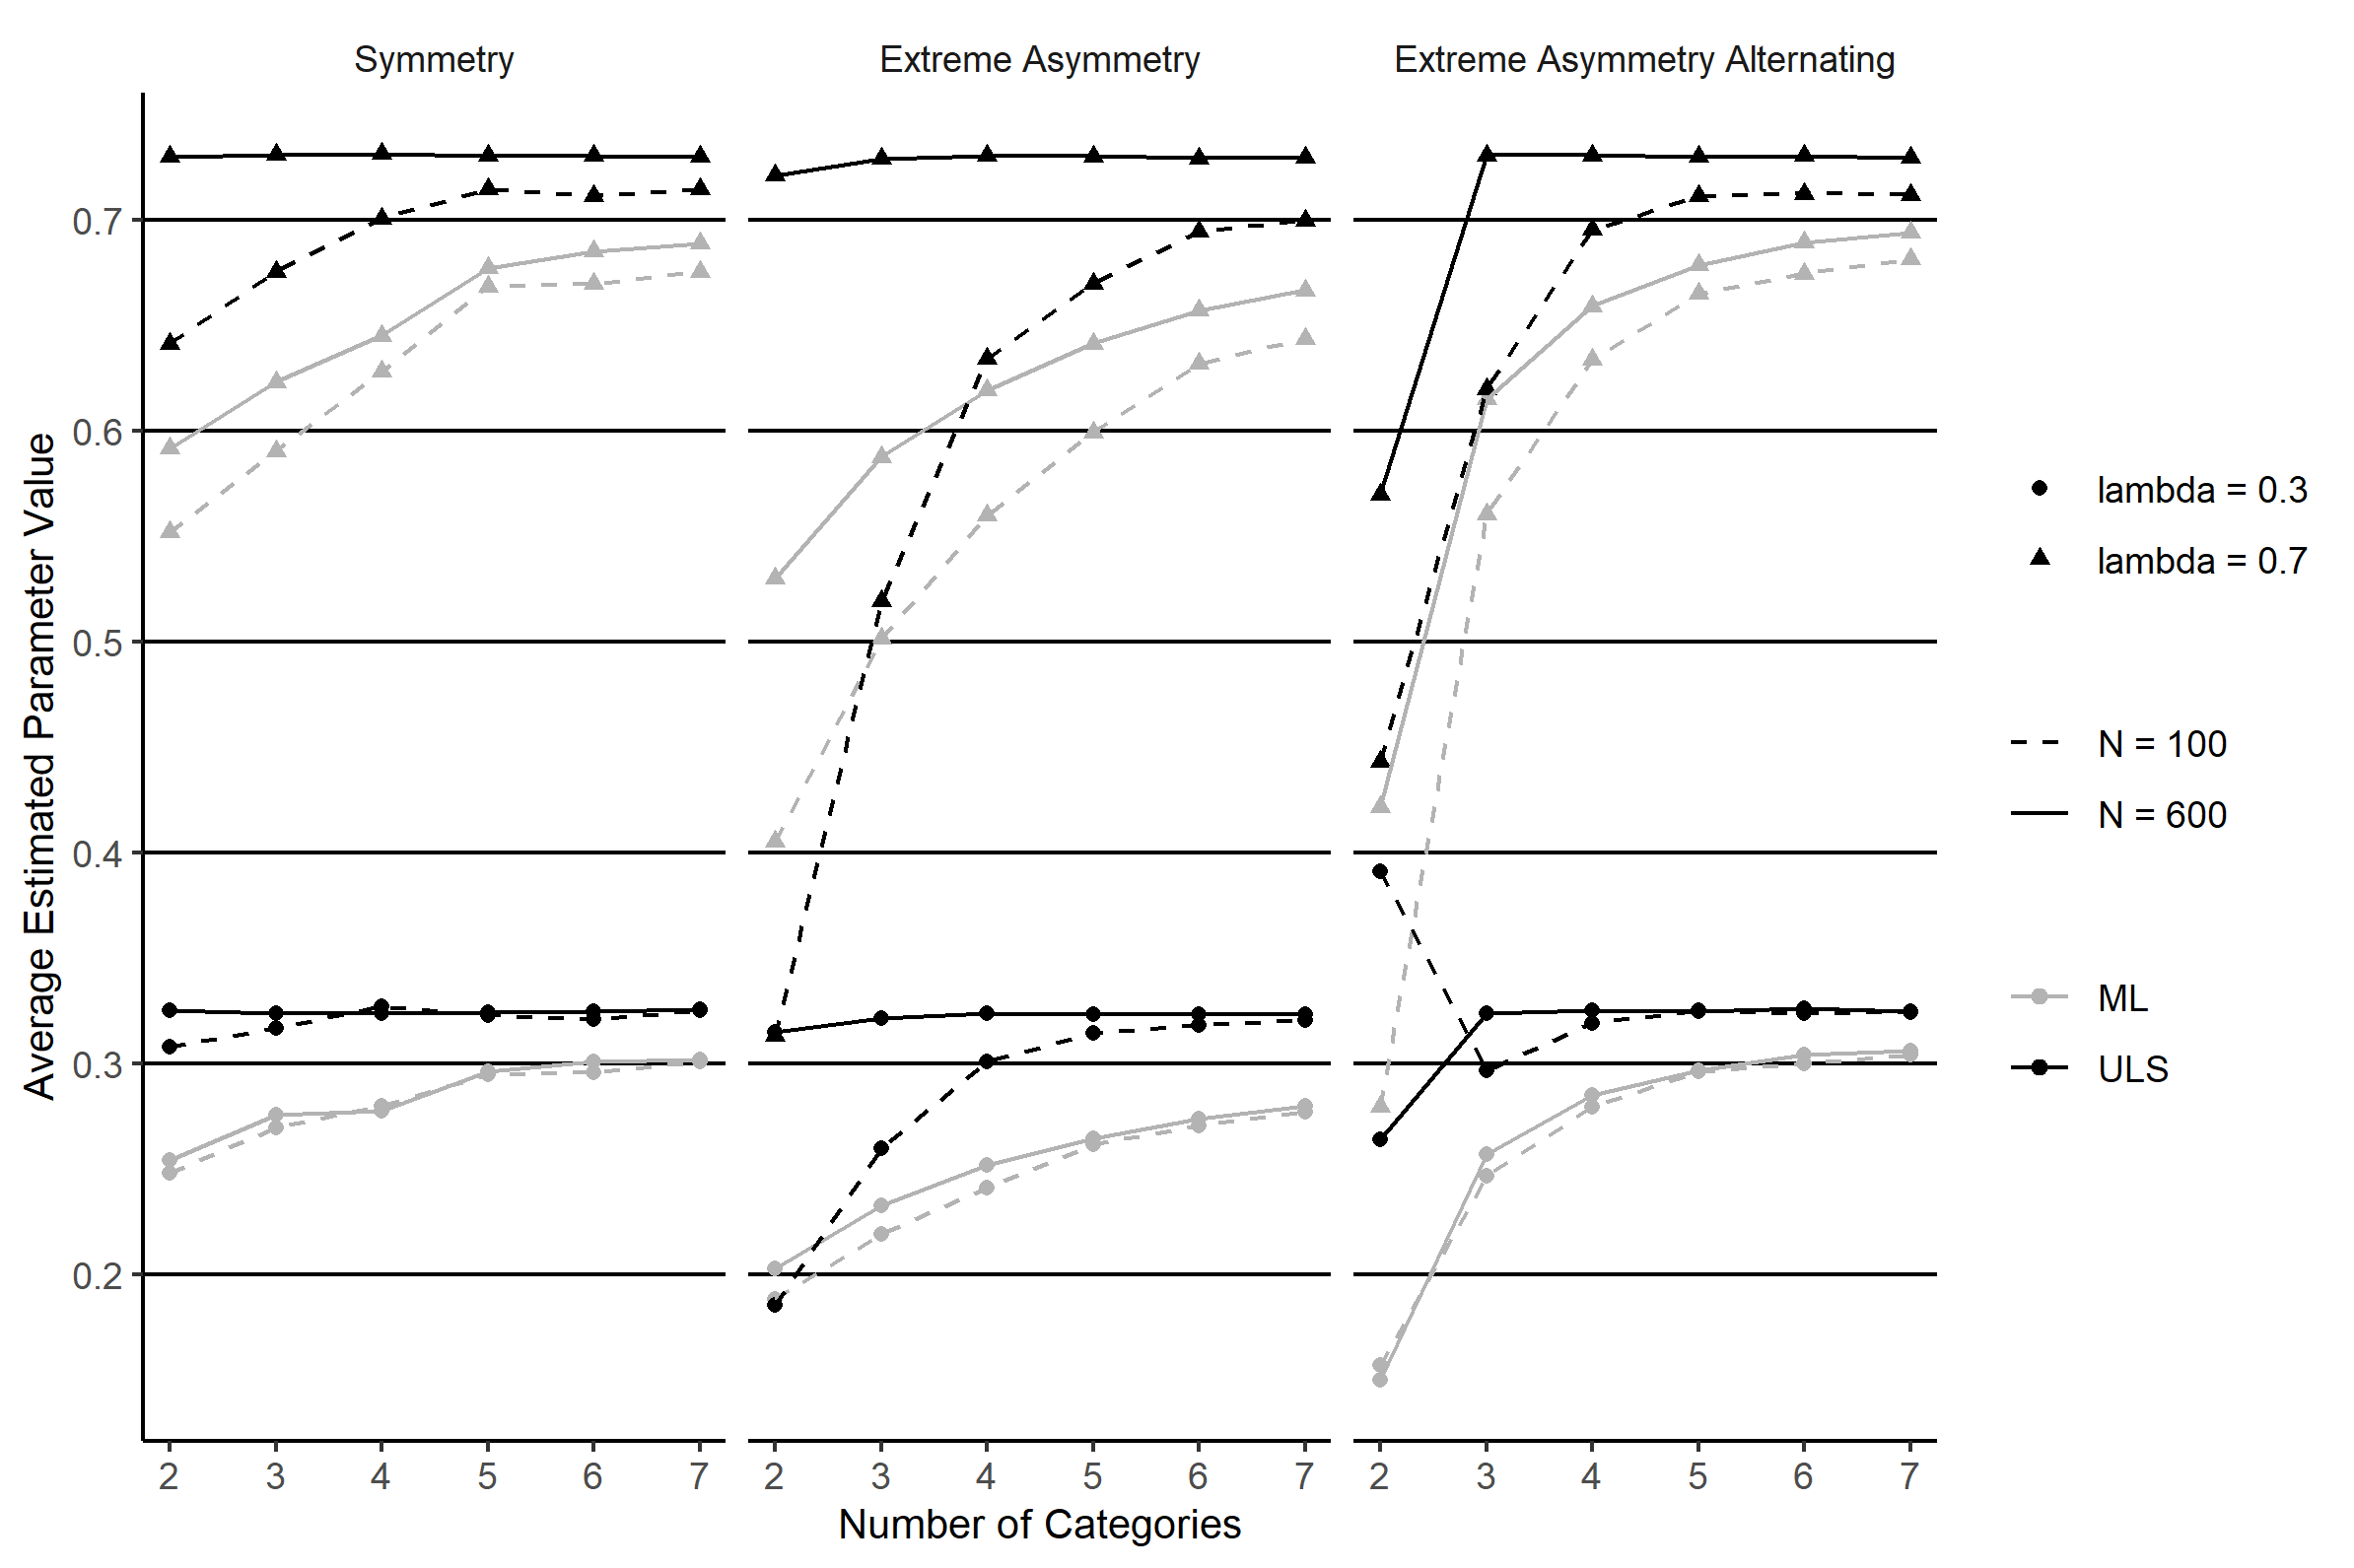
\includegraphics[width=0.49\linewidth]{./figures/fig_4} 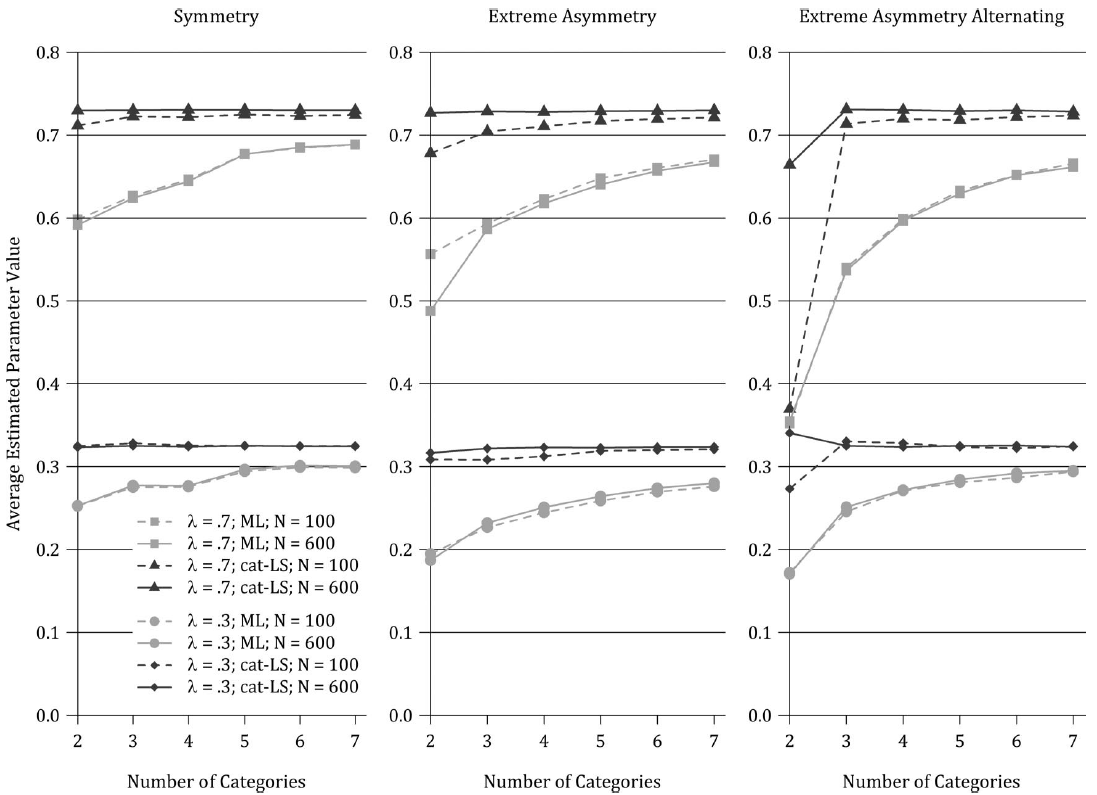
\includegraphics[width=0.49\linewidth]{./figures/fig4_original} \caption{Parameter estimates (factor loadings, underlying distribution is nonnormal; skew 2, kurtosis 7). Values are averaged across model size and across all loadings for which the true parameter value was the same. Lines represent different estimators and different sample sizes (see legend). ML = robust continuous maximum likelihood estimation; cat-LS = robust categorical least squares estimation. The upper set of lines represents results for a true parameter value of .7. The lower set of lines represents results for a true parameter value of .3. Vertical panels represent different levels of threshold symmetry. Left figure: replication; right figure original study.}\label{fig:fig4}
\end{figure}

\subsubsection{Figure 5 Parameter estimates (factor correlation)}

\begin{figure}
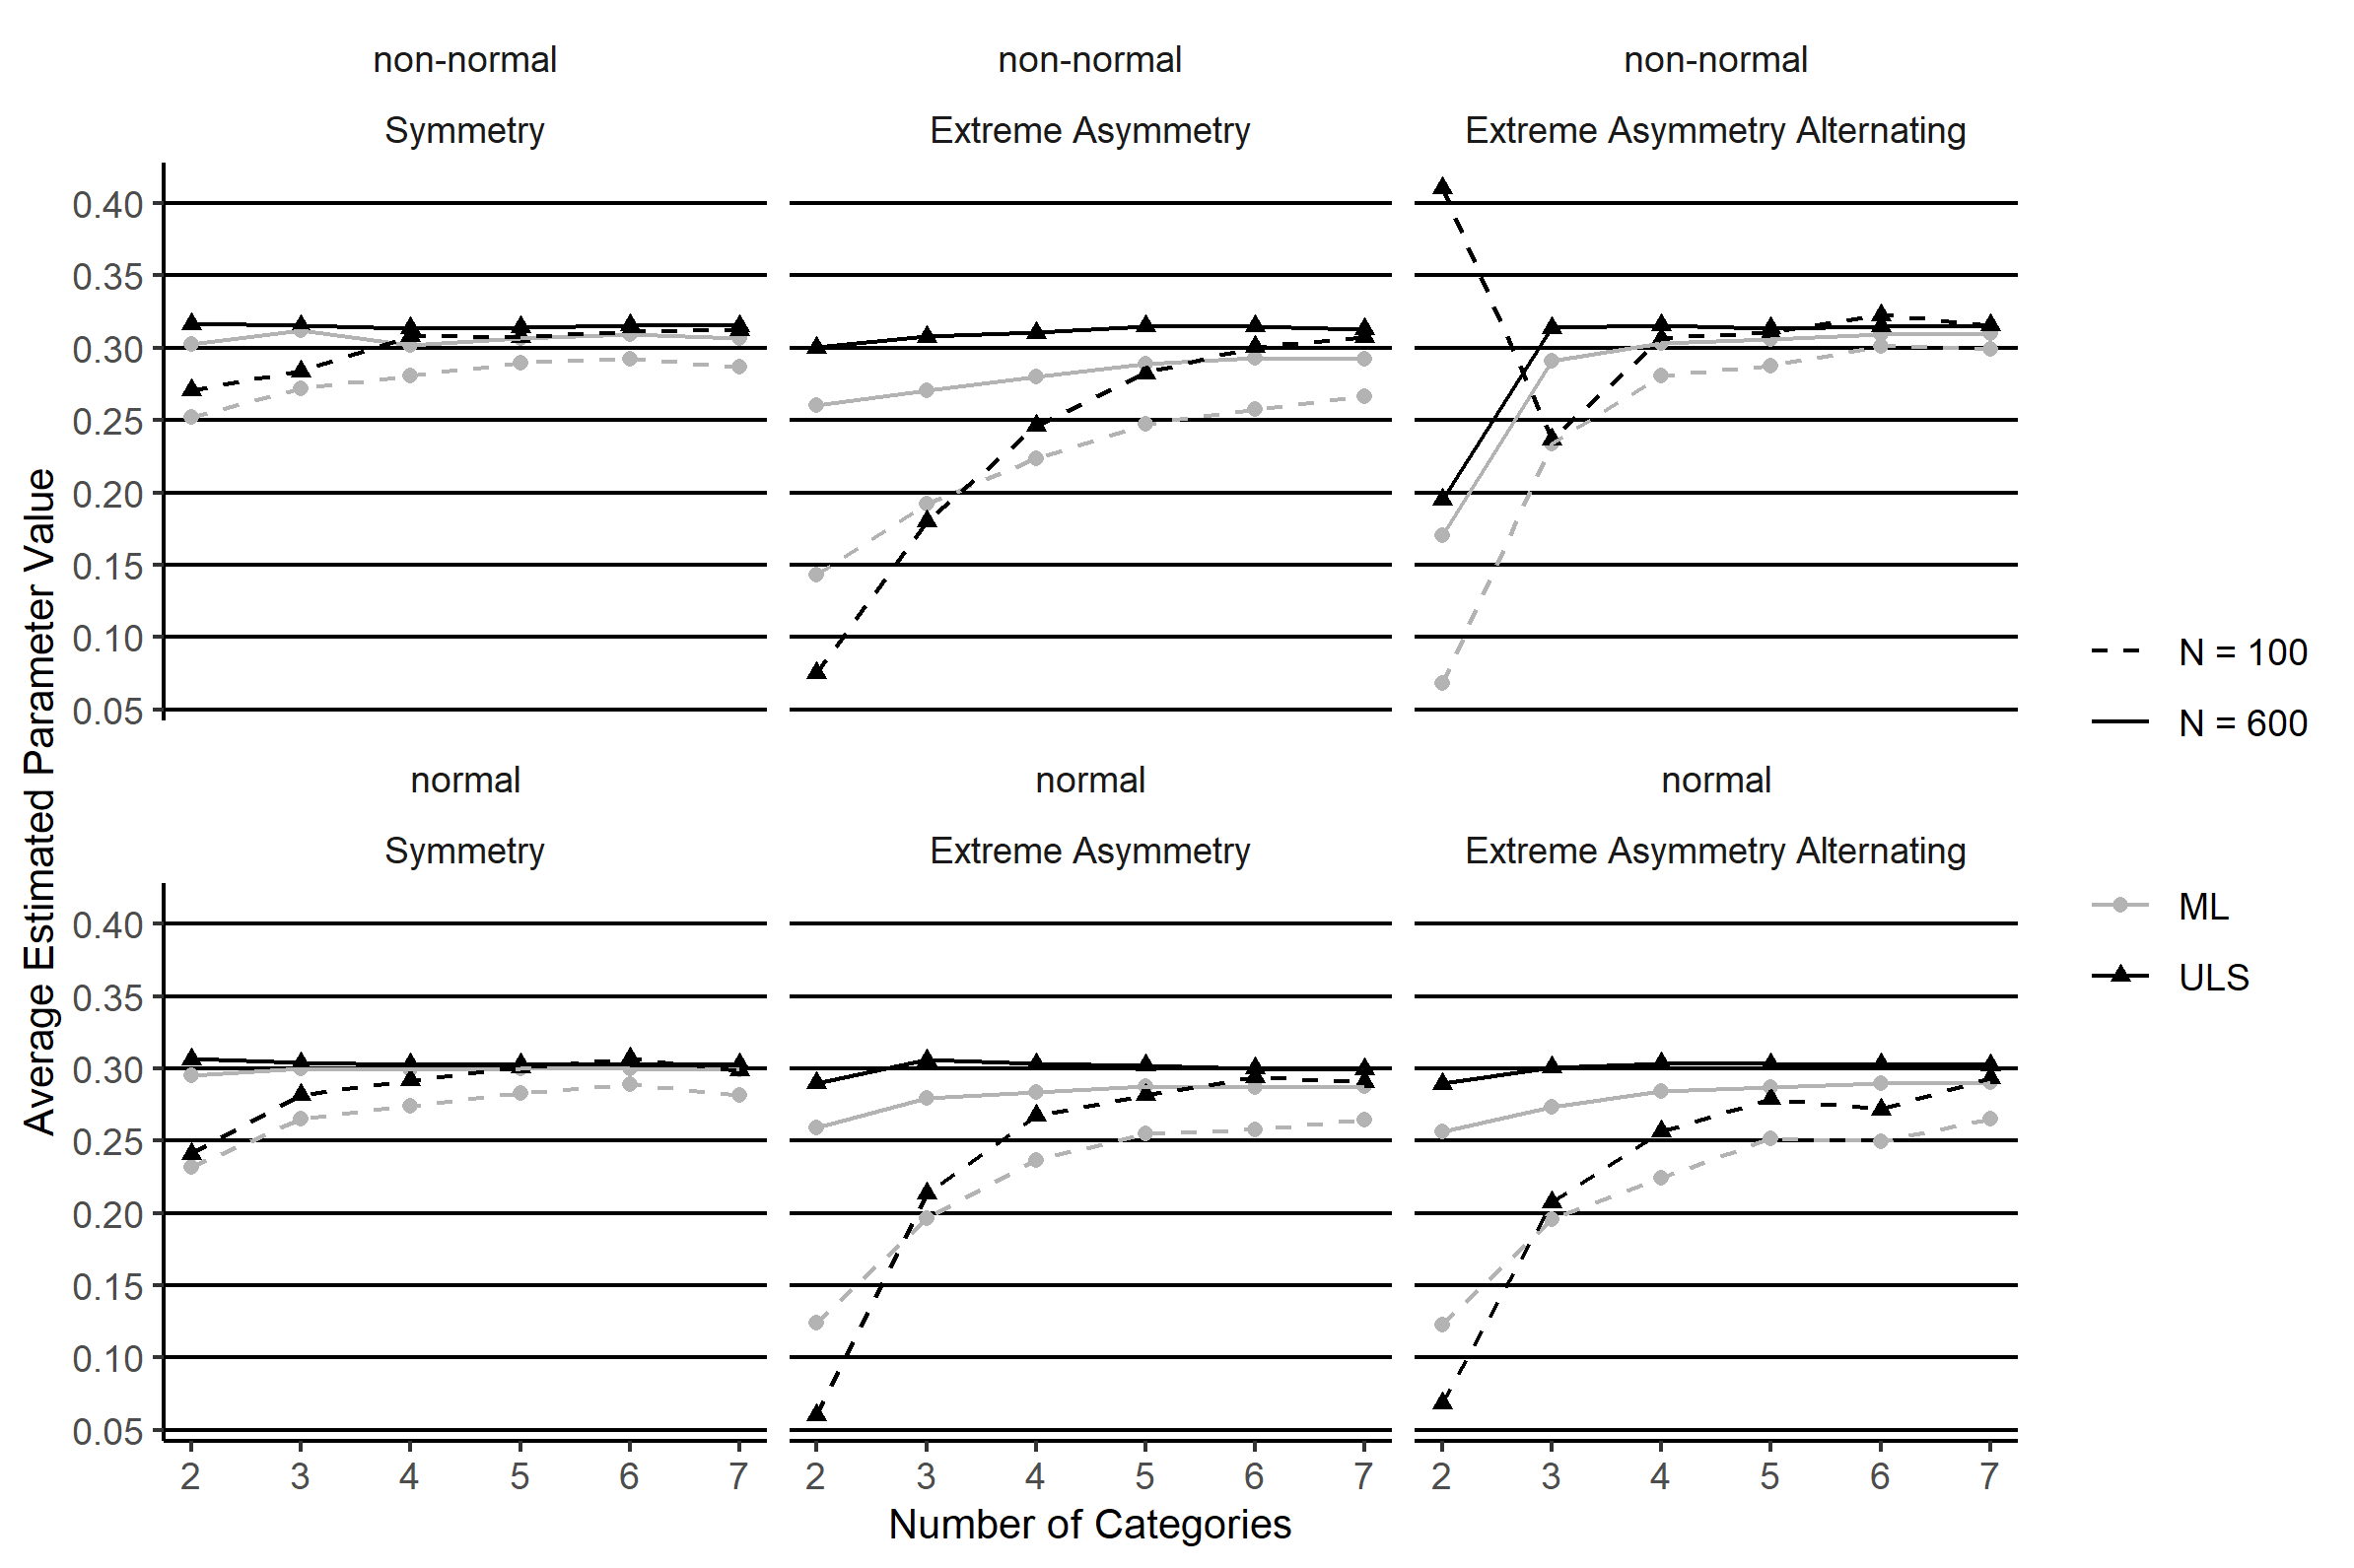
\includegraphics[width=0.49\linewidth]{./figures/fig_5} 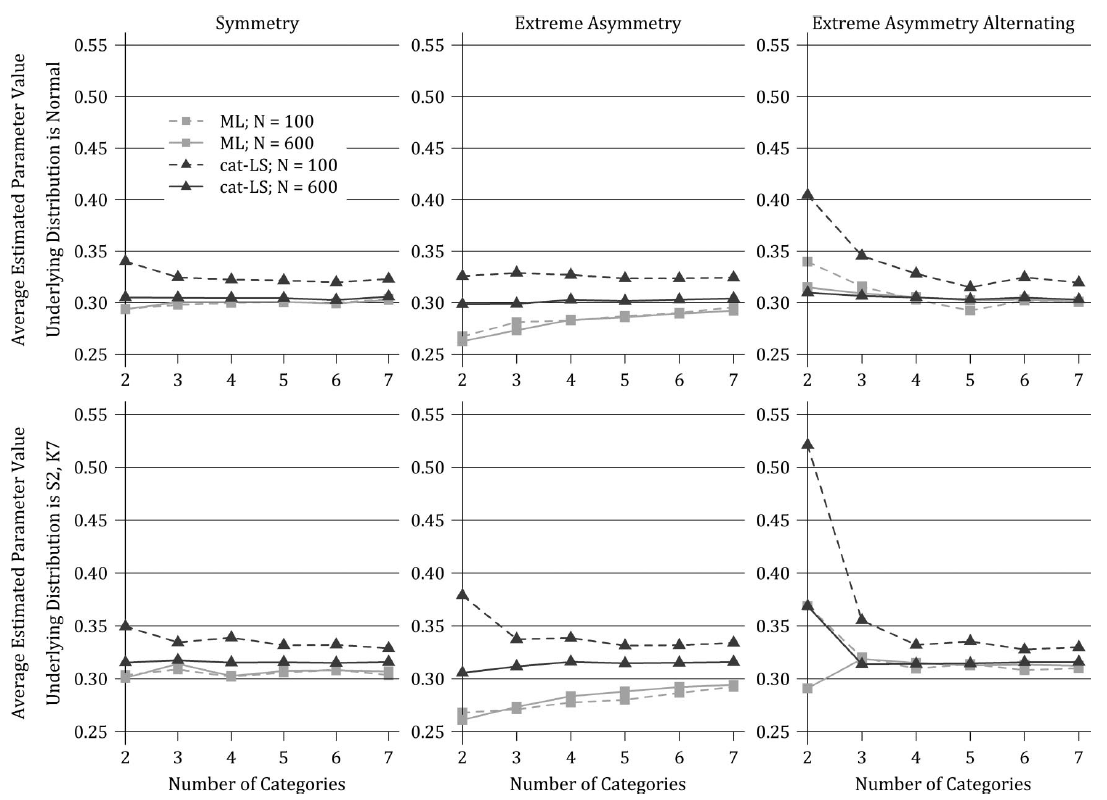
\includegraphics[width=0.49\linewidth]{./figures/fig5_original} \caption{Parameter estimates (factor correlation, true value is .3). Values are averaged across model size. Lines represent different estimators and different sample sizes (see legend). ML = robust continuous maximum likelihood estimation; cat-LS = robust categorical least squares estimation. The upper panel corresponds to conditions in which the underlying distribution is normal; the lower panel corresponds to conditions in which the underlying distribution is nonnormal (skew 2, kurtosis 7). Vertical panels represent different levels of threshold symmetry. Left figure: replication; right figure original study.}\label{fig:fig5}
\end{figure}

Parameter estimates for the factor correlations largely align with the
original results. For scenarios where \emph{N} = 100, we observed a
larger downwards bias, especially for scenarios with a low number of
categories.

\subsubsection{Figure 6 and 7 Coverage (factor loadings)}

\begin{figure}
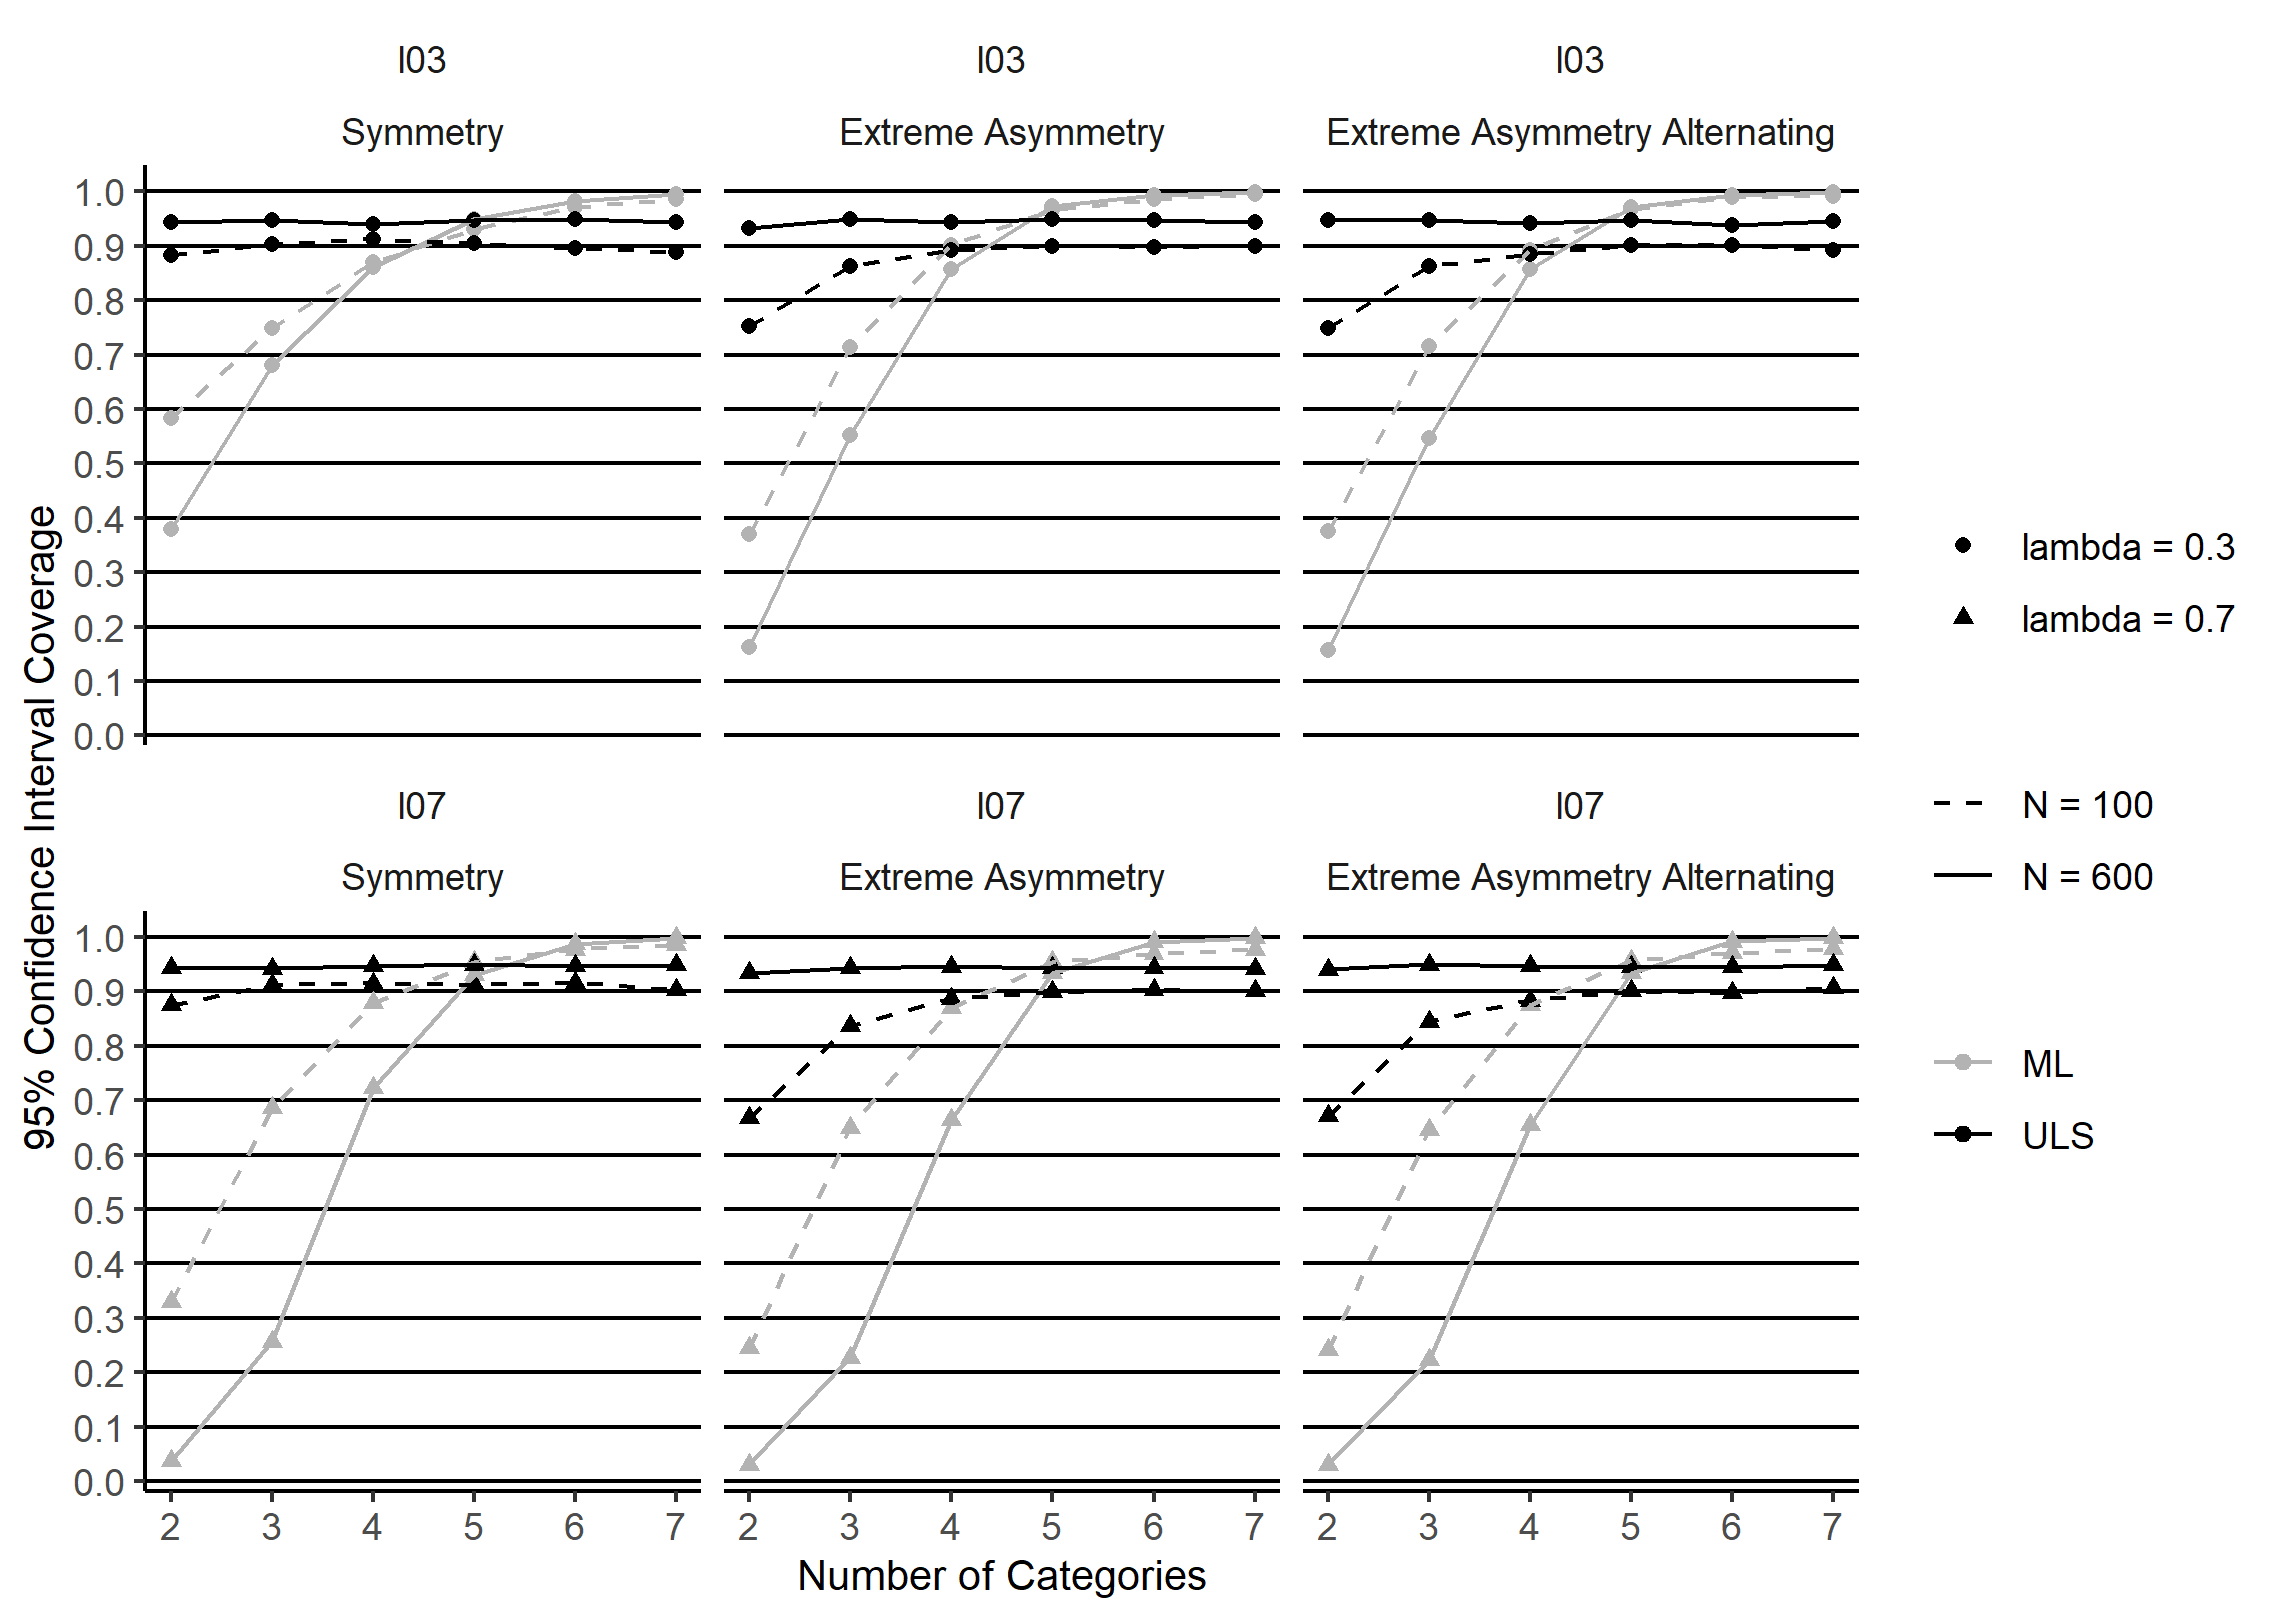
\includegraphics[width=0.49\linewidth]{./figures/fig_6} 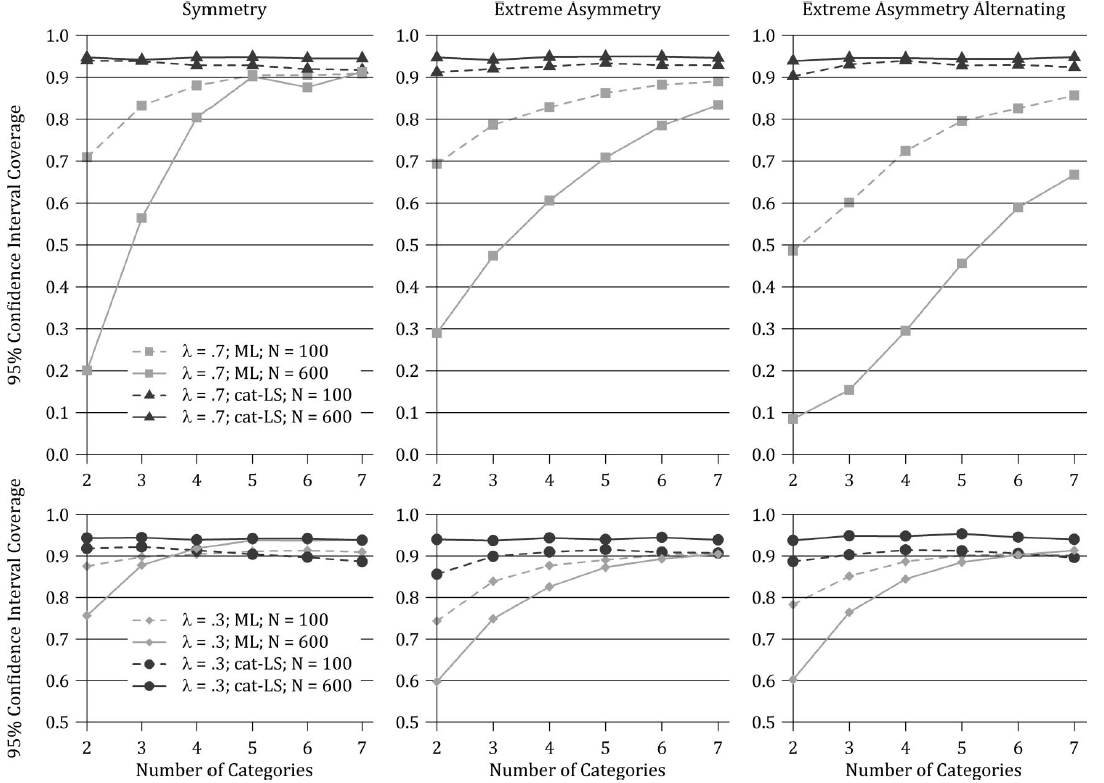
\includegraphics[width=0.49\linewidth]{./figures/fig6_original} \caption{Coverage by number of categories (.7 and .3 factor loadings); underlying distribution is normal. Values are averaged across model size and across all loadings for which the true parameter value was the same. Lines represent different estimators and different sample sizes (see legend). ML = robust continuous maximum likelihood estimation; cat-LS = robust categorical least squares estimation. The upper panel represents results for a true parameter value of .7. The lower panel represents results for a true parameter value of .3. Vertical panels represent different levels of threshold symmetry. Left figure: replication; right figure original study.}\label{fig:fig6}
\end{figure}

\begin{figure}
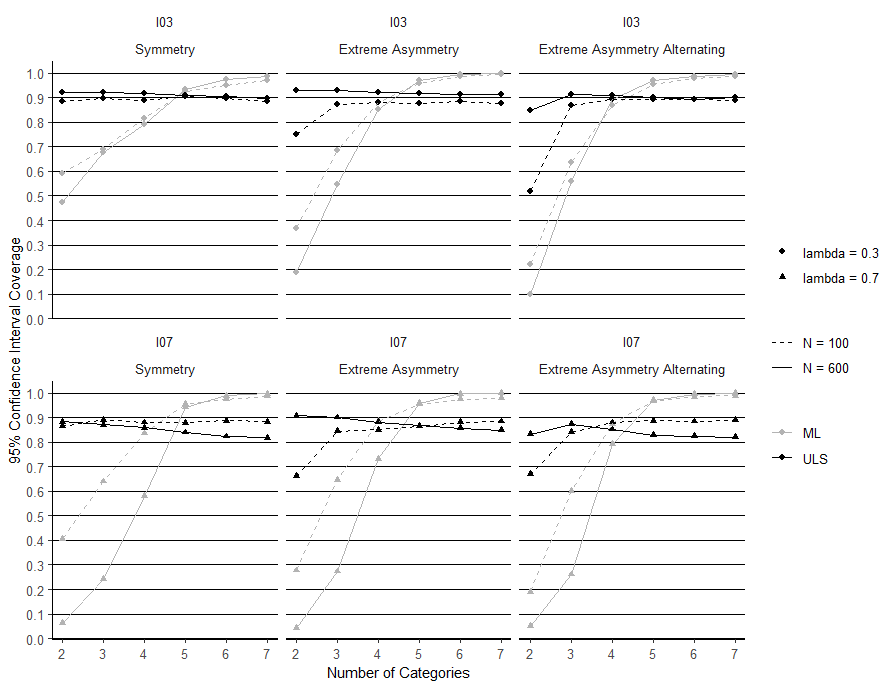
\includegraphics[width=0.49\linewidth]{./figures/fig7} 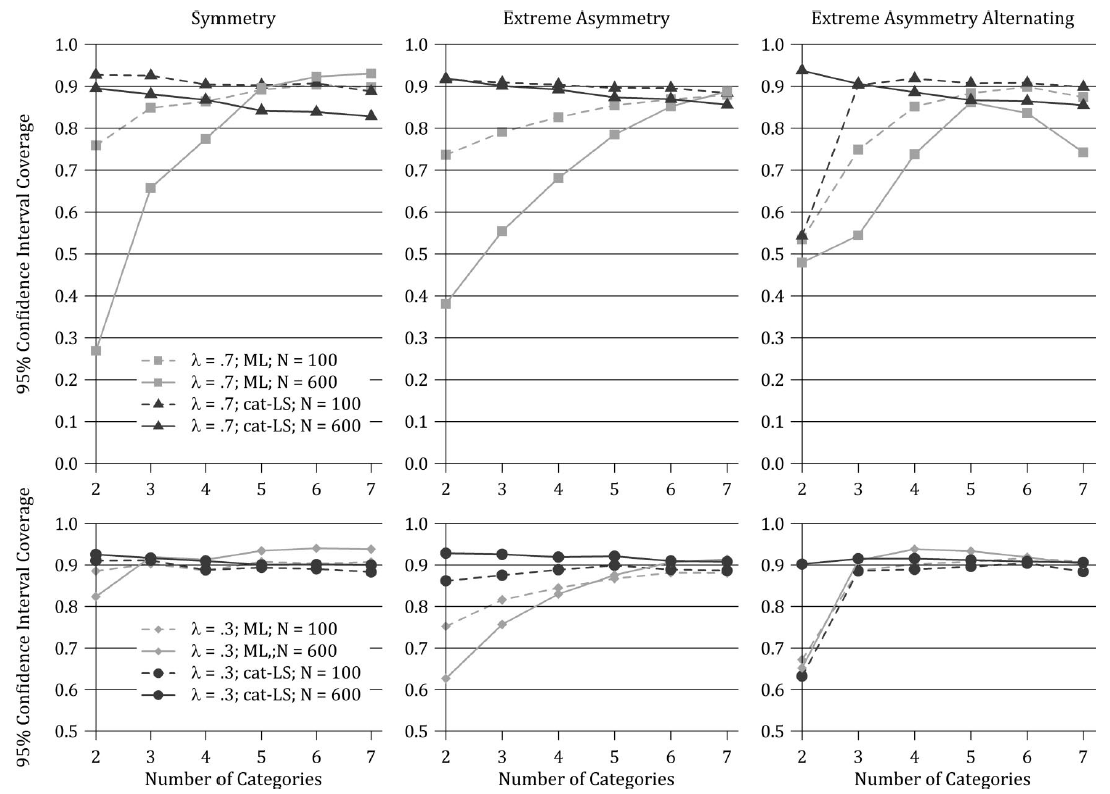
\includegraphics[width=0.49\linewidth]{./figures/fig7_original} \caption{Coverage by number of categories (.7 and .3 factor loadings); underlying distribution is nonnormal (skew 2, kurtosis 7). Values are averaged across model size, and across all loadings for which the true parameter value was the same. Lines represent different estimators and different sample sizes (see legend). ML = robust continuous maximum likelihood estimation; cat-LS = robust categorical least squares estimation. The upper panel represents results for a true parameter value of .7. The lower panel represents results for a true parameter value of .3. Vertical panels represent different levels of threshold symmetry. Left figure: replication; right figure original study.}\label{fig:fig7}
\end{figure}

Regarding coverage the trends in our results correspond to the original
findings. Regarding magnitude, our results show consistently lower
coverage especially with ML estimator and lower number of categories.

\subsubsection{Figure 8 Coverage (factor correlations)}

\begin{figure}
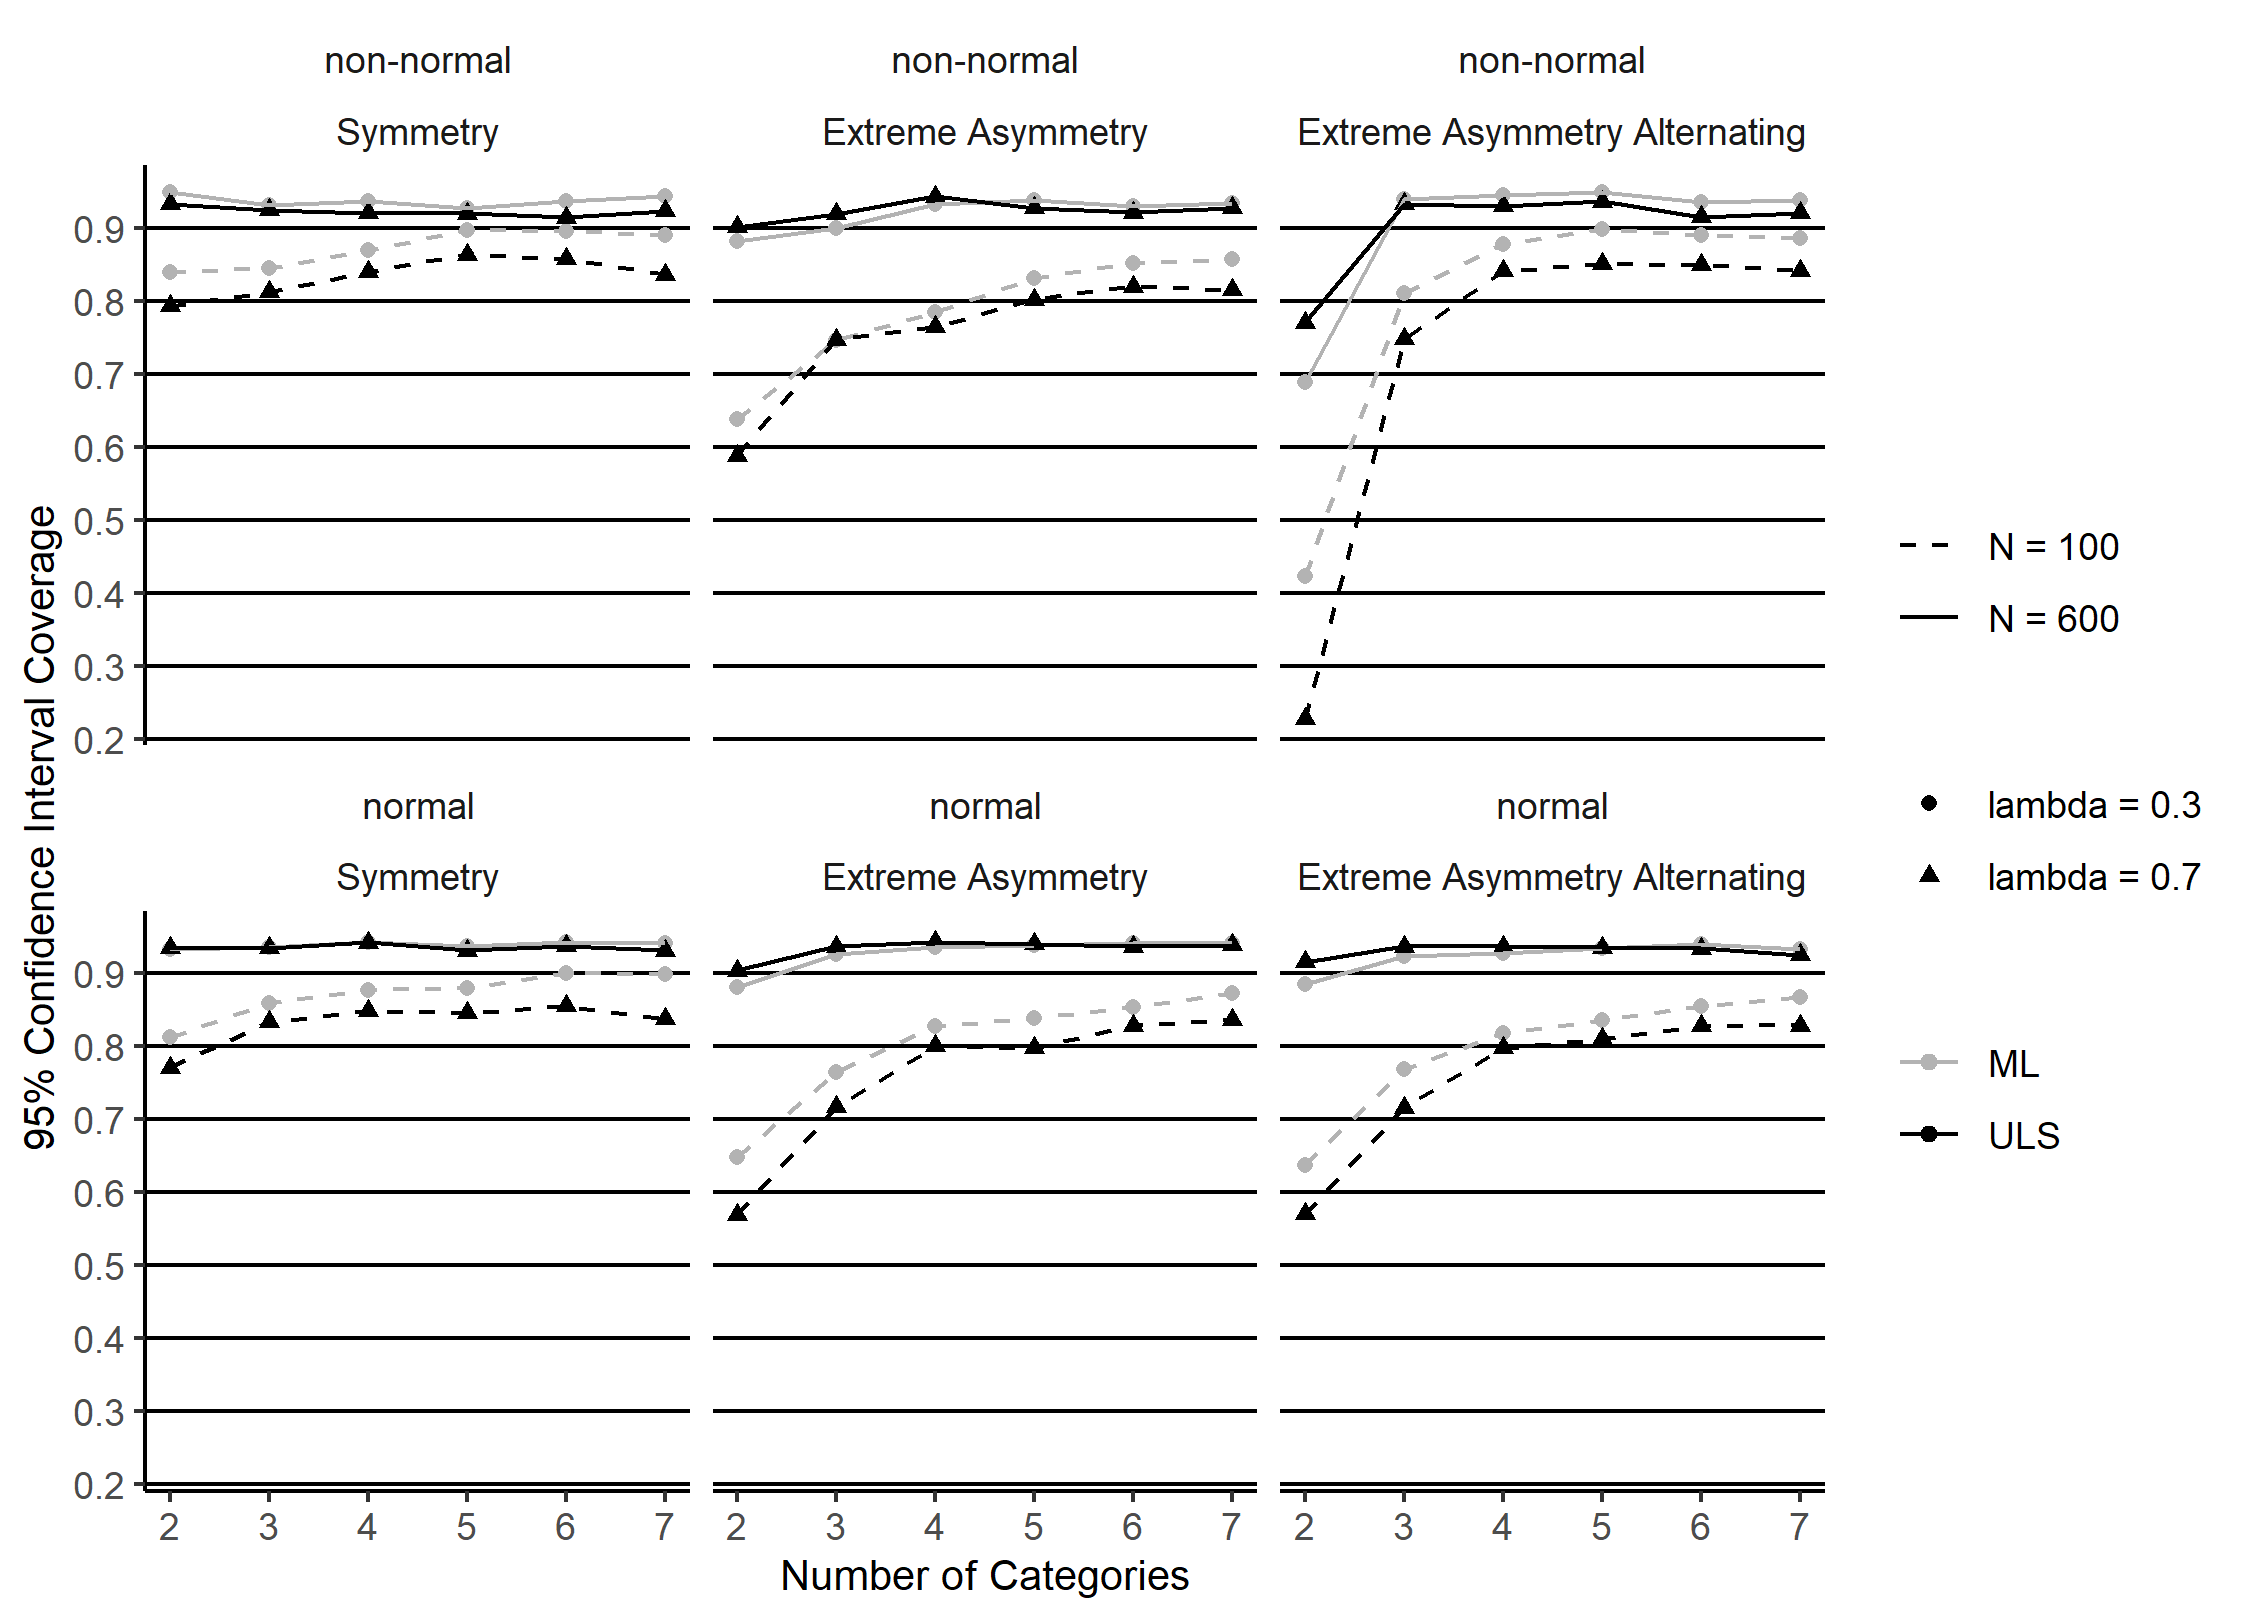
\includegraphics[width=0.49\linewidth]{./figures/fig_8} 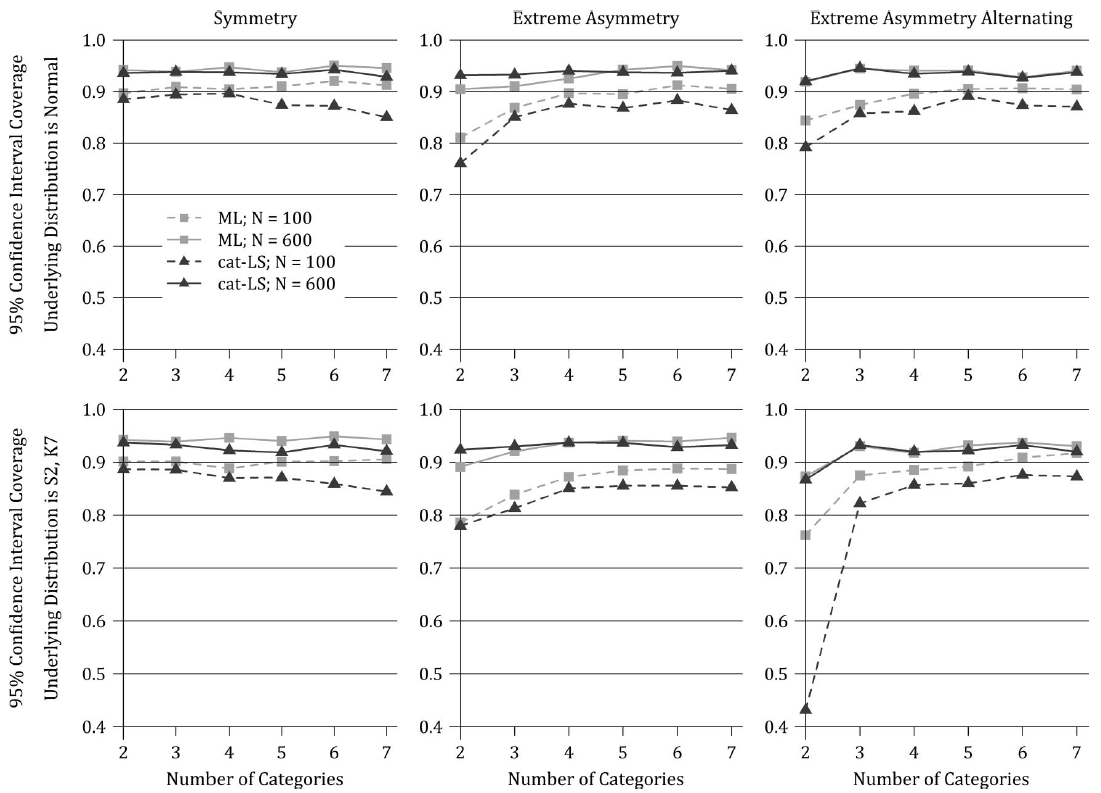
\includegraphics[width=0.49\linewidth]{./figures/fig8_original} \caption{Coverage by number of categories (factor correlation). Values are averaged across model size. Lines represent different estimators and different sample sizes (see legend). ML = robust continuous maximum likelihood estimation; cat-LS = robust categorical least squares estimation. The upper panel corresponds to conditions in which the underlying distribution is normal; the lower panel corresponds to conditions in which the underlying distribution is nonnormal (skew 2, kurtosis 7). Vertical panels represent different levels of threshold symmetry. Left figure: replication; right figure original study.}\label{fig:fig8}
\end{figure}

Type I error of mean-and variance adjusted test statistic roughly aligns
for symmetry and extreme asymmetry scenarios. In the Extreme Asymmetry
Alternating scenarios the original study finds considerably higher type
I error rates for scenarios pertaining to the ML estimator and \emph{N}
= 600.

Regarding coverage of the factor correlation our results closely align
with the original findings considering trends. Considering magnitude,
coverage in the N=100 scenarios is consistently lower.

\subsubsection{Type I error rate}
\begin{figure}
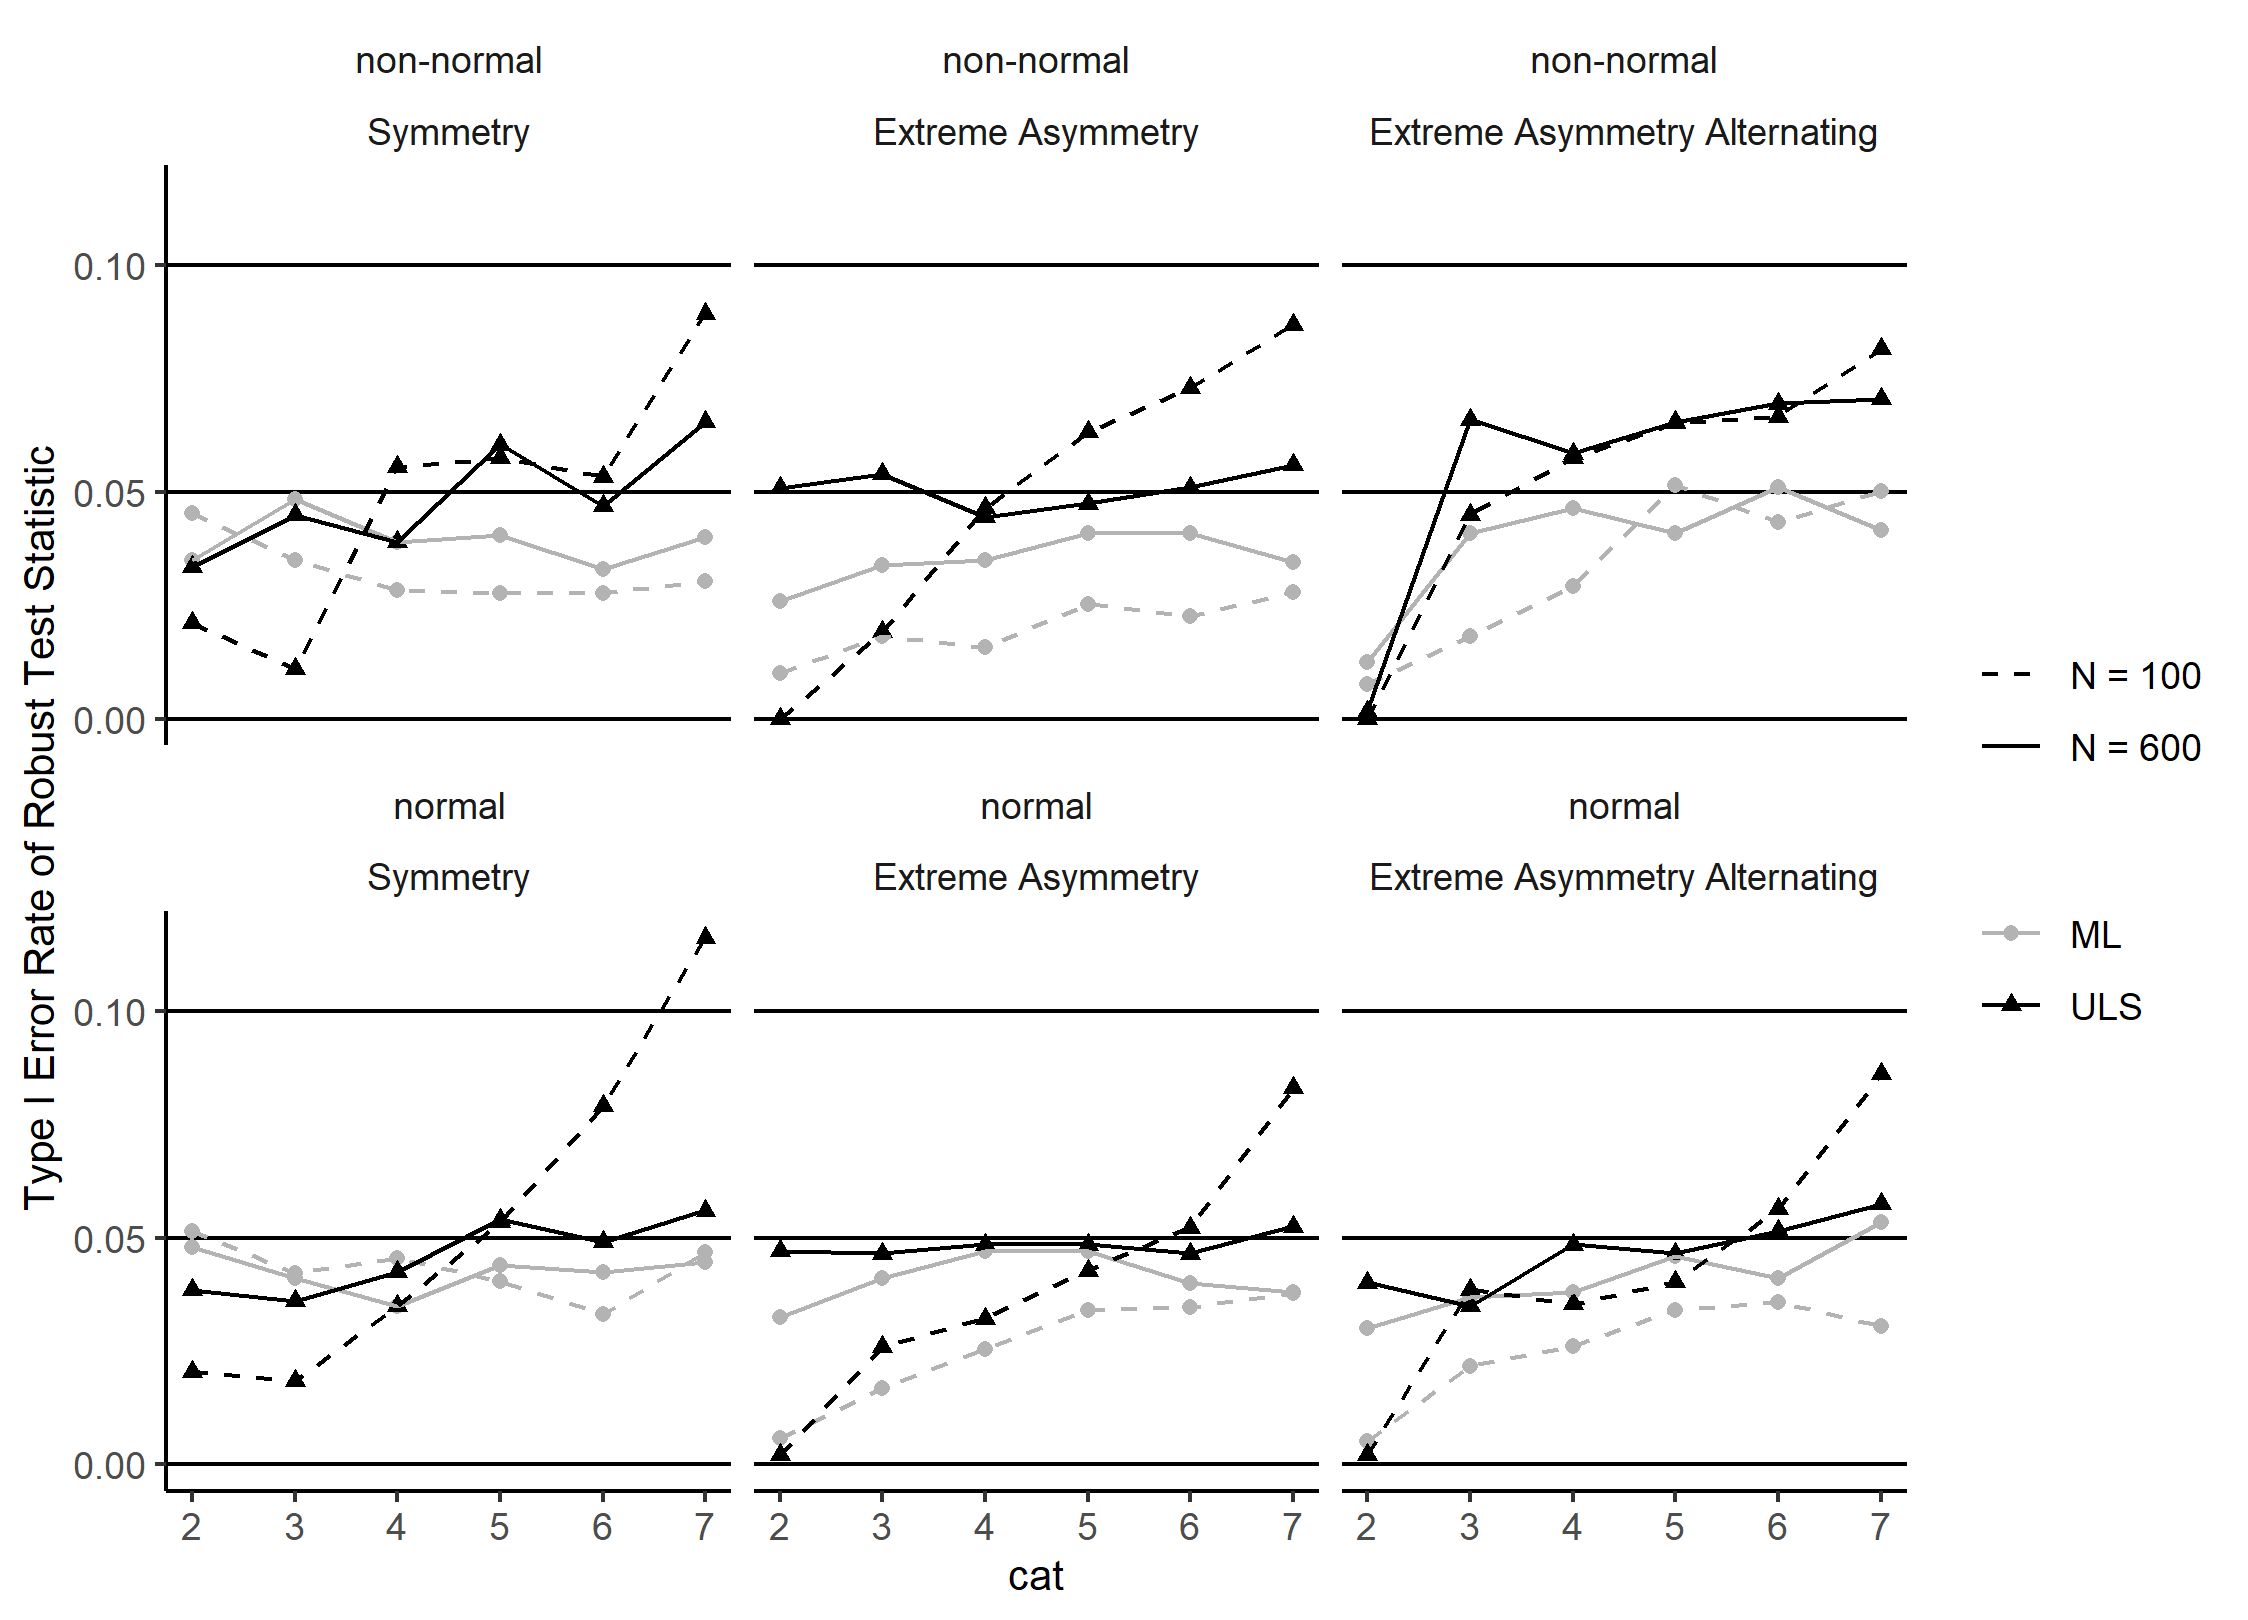
\includegraphics[width=0.49\linewidth]{./figures/fig_9} 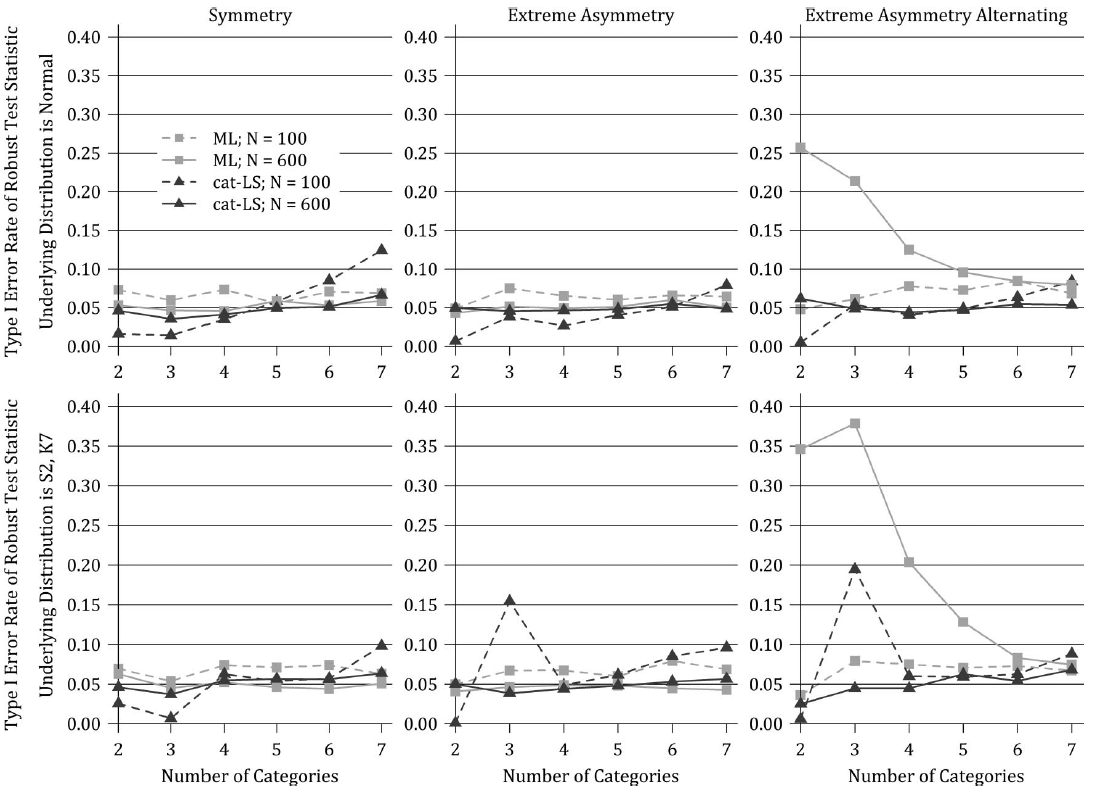
\includegraphics[width=0.49\linewidth]{./figures/fig9_original} \caption{Type I error of mean-and-variance adjusted test statistic by number of categories. Values are averaged across model size. Lines represent different estimators and different sample sizes (see legend). ML = robust continuous maximum likelihood estimation; cat-LS = robust categorical least squares estimation. The upper panel corresponds to conditions in which the underlying distribution is normal; the lower panel corresponds to conditions in which the underlying distribution is nonnormal (skew 2, kurtosis 7). Vertical panels represent different levels of threshold symmetry.}\label{fig:fig9}
\end{figure}

\subsection{Replication of result tables}

\subsubsection{Table 1}

Table 1 presents the \emph{``Skew and Kurtosis of Observed Categorical
Variables by Threshold Distribution, Underlying Distribution, and Number
of Categories''} (p.~363). The \emph{``{[}v{]}alues in this table were
obtained by generating samples of size N = 1,000,000 for each condition
and recording the skew and kurtosis of the observed distributions.''}
(p.~363) As discussed above we understood ``each condition'' to only
include underlying distribution, number of categories and threshold
symmetry. We hence only simulated one variable of sample size 1,000,000
per condition in order to replicate Figure 1, Figure 2 as well as Table
1.

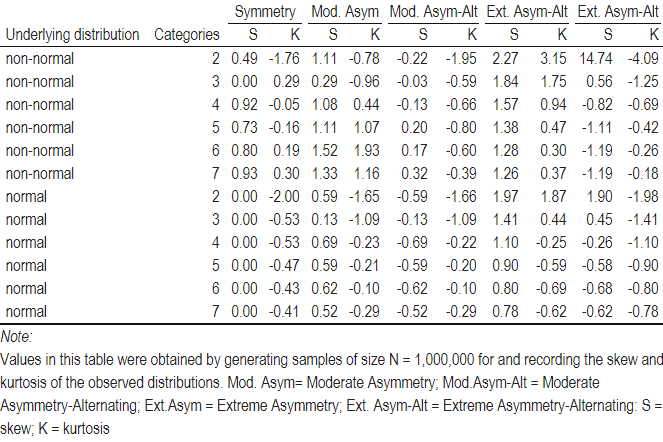
\includegraphics[width=385pt]{./figures/table1}

\subsubsection{Observed Power (Table 2)}

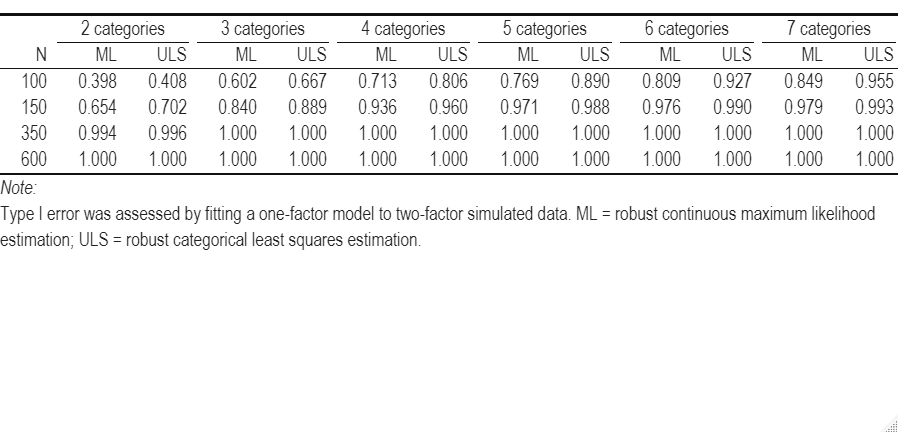
\includegraphics[width=385pt]{./figures/table2}

Results regarding observed power closely aligned with the original
findings. The scenarios exhibiting a power below .8 matched the ones
identified in the original study.

\subsection{Replication of supplemental results}

The following tables correspond to tables presented in the supplemental
material of the original study which can be accessed at
\url{http://dx.doi.org/10.1037/a0029315.supp}

\subsubsection{Number of nonconverged cases per 1000 replications (A2/A3)}

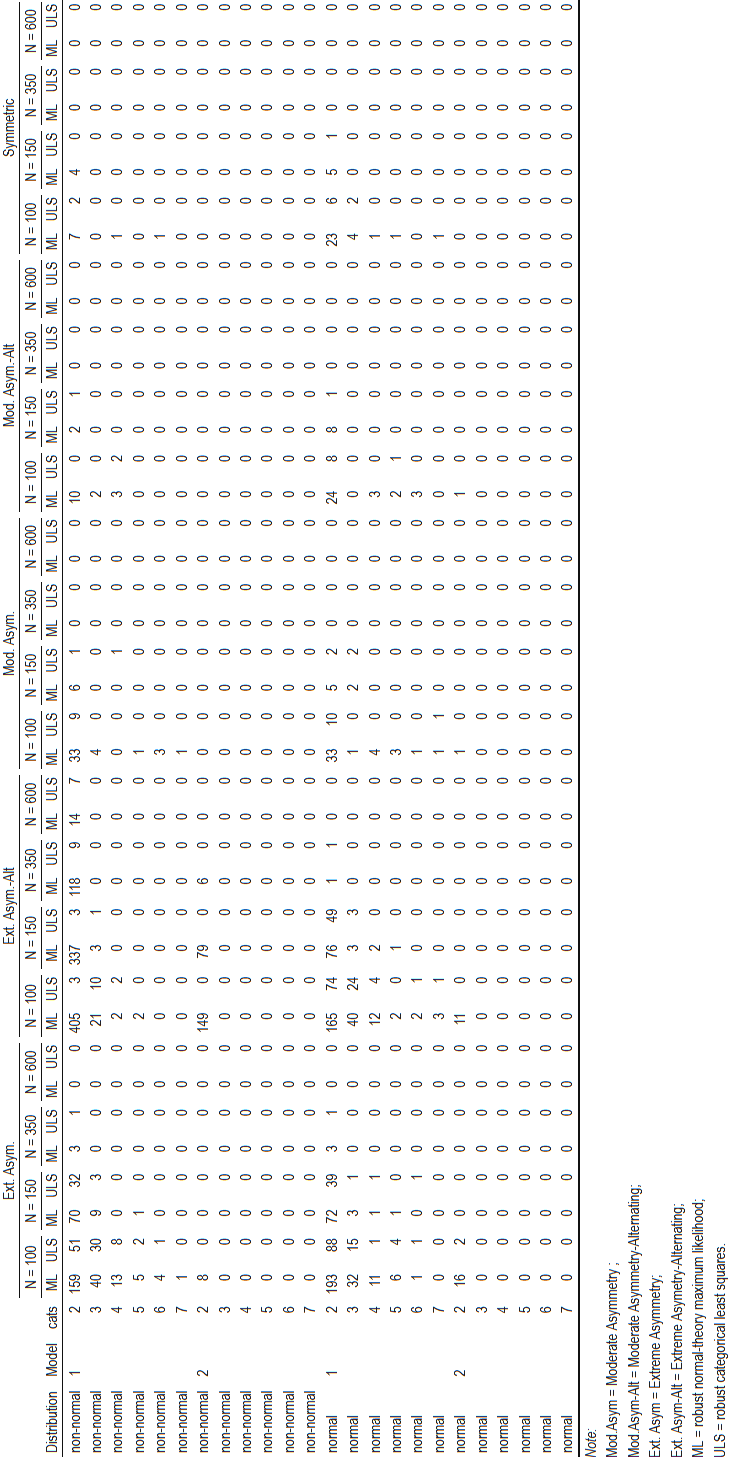
\includegraphics[width=315pt]{./figures/tabA2_A3}

\subsubsection{Number of improper solutions per 1000 replications (A4/A5)}

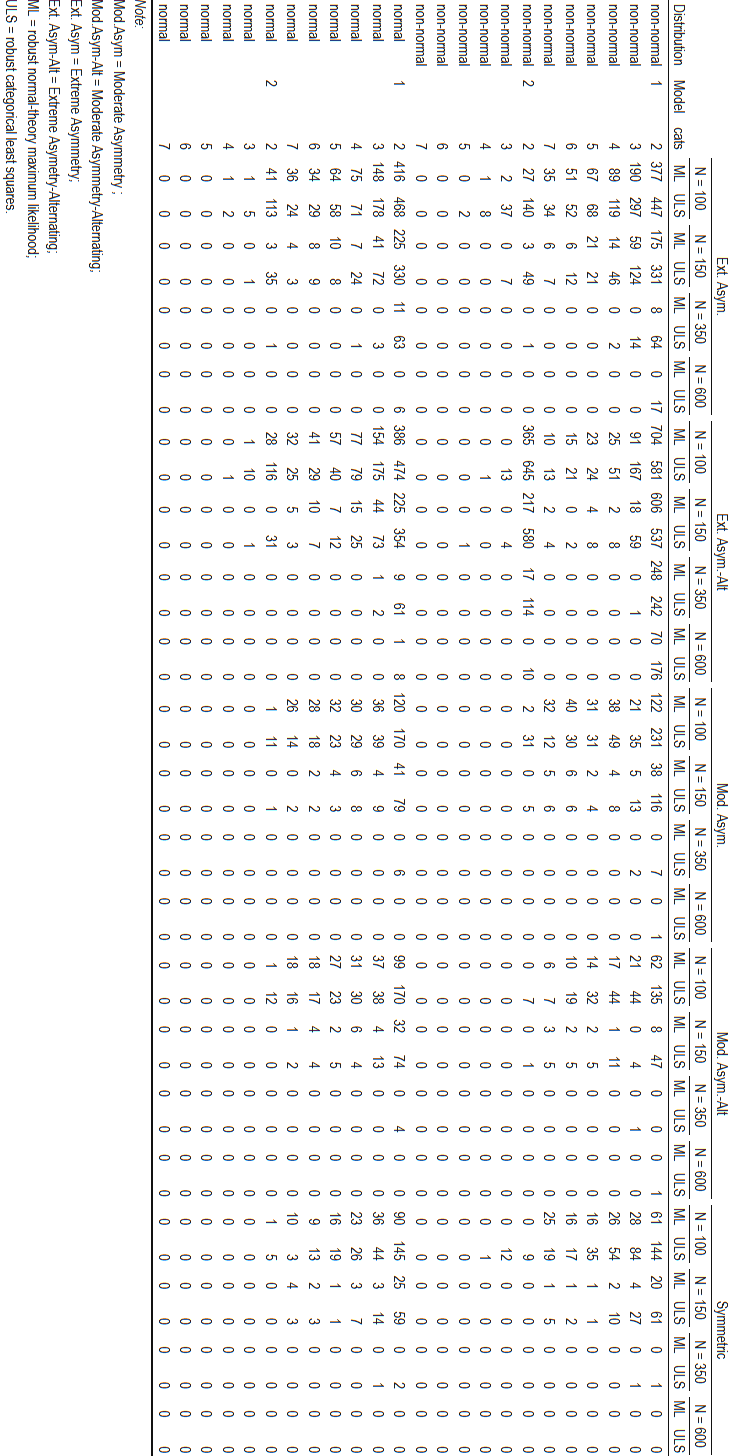
\includegraphics[width=315pt]{./figures/tabA4_A5}

\subsubsection{Parameter Bias, Model1, Underlying Distribution = Normal (A6)}

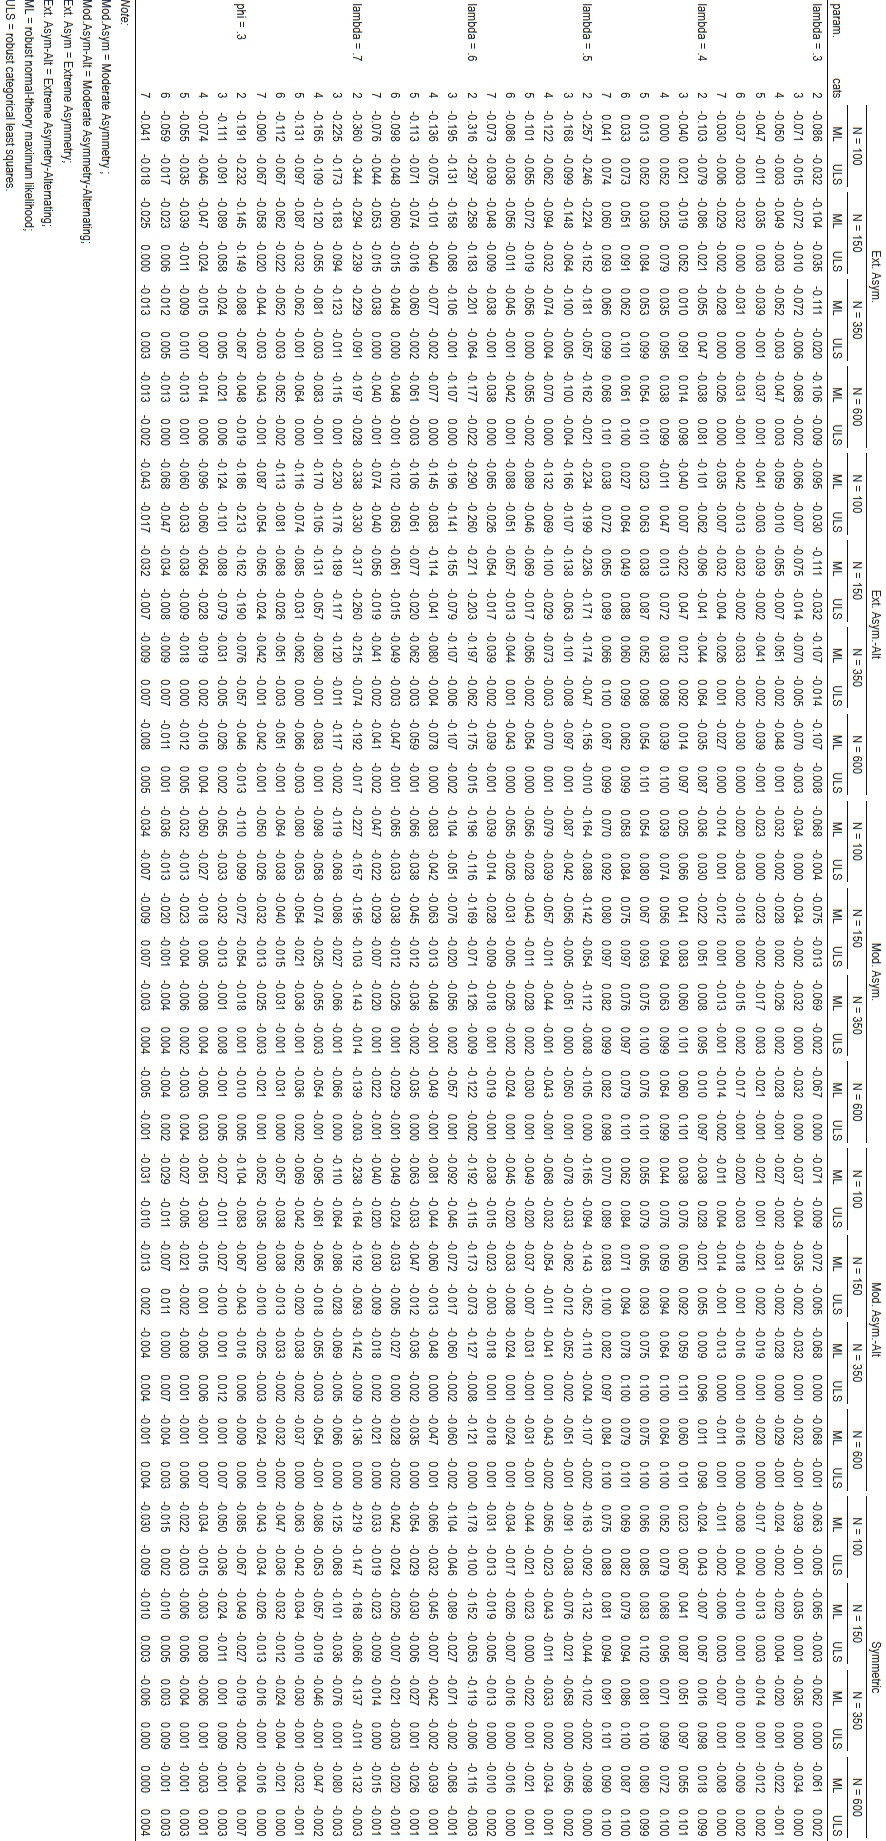
\includegraphics[width=325pt]{./figures/tabA6}

\subsubsection{Parameter Bias, Model1, Underlying Distribution = Skew 2, Kurtosis 7 (A7)}

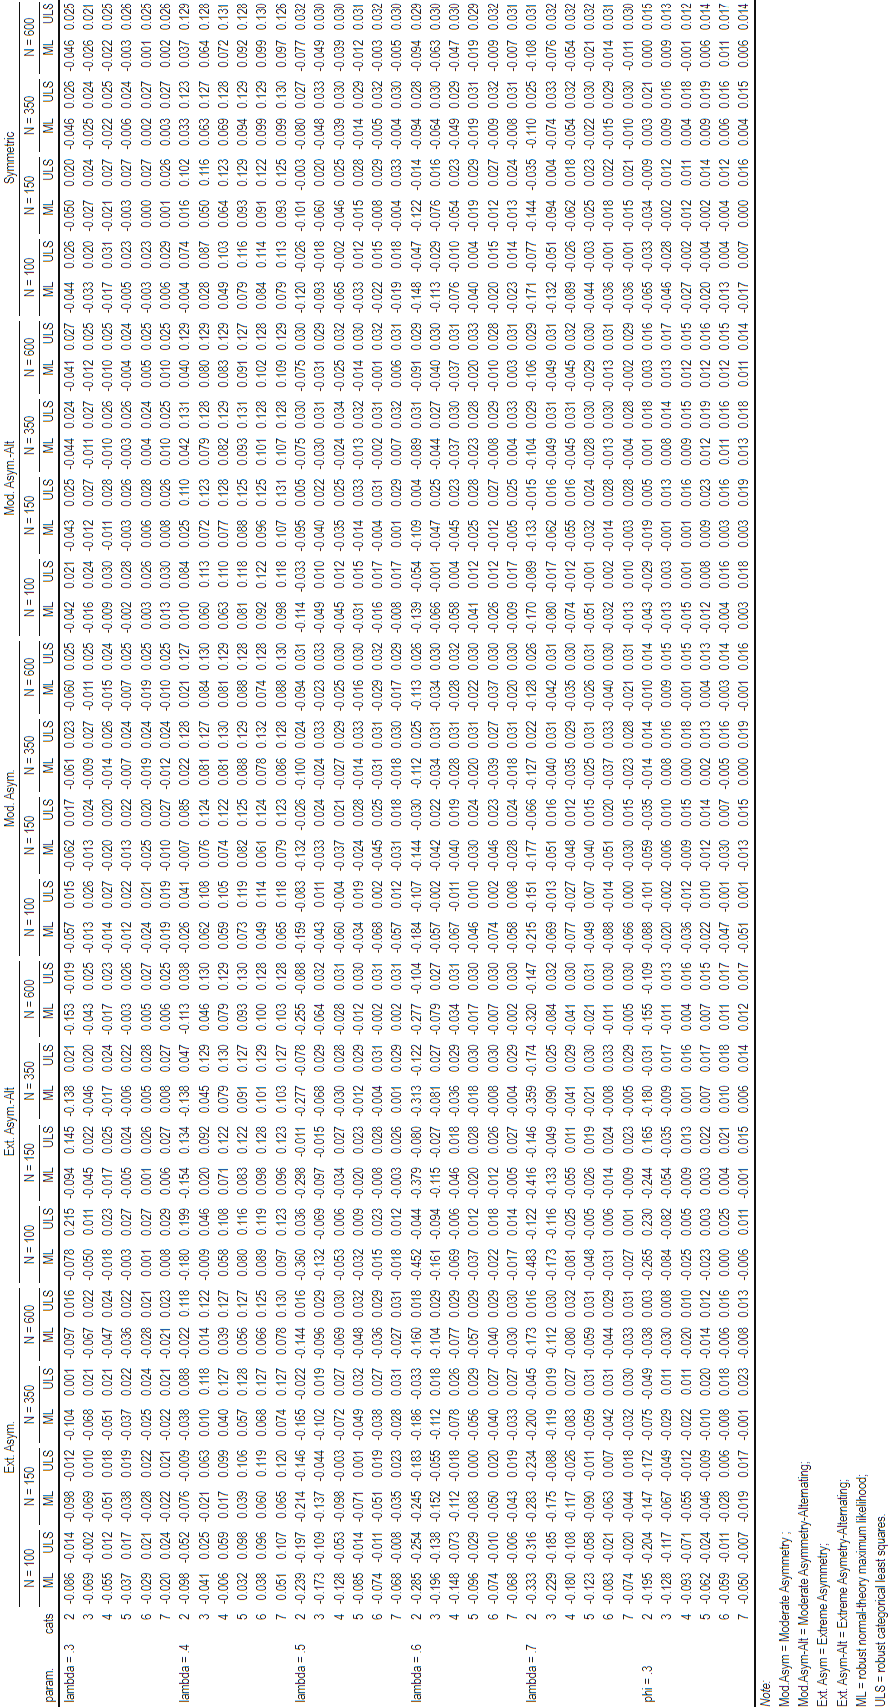
\includegraphics[width=325pt]{./figures/tabA7}

\subsubsection{Parameter Bias, Model2, Underlying Distribution = Normal (A8)}

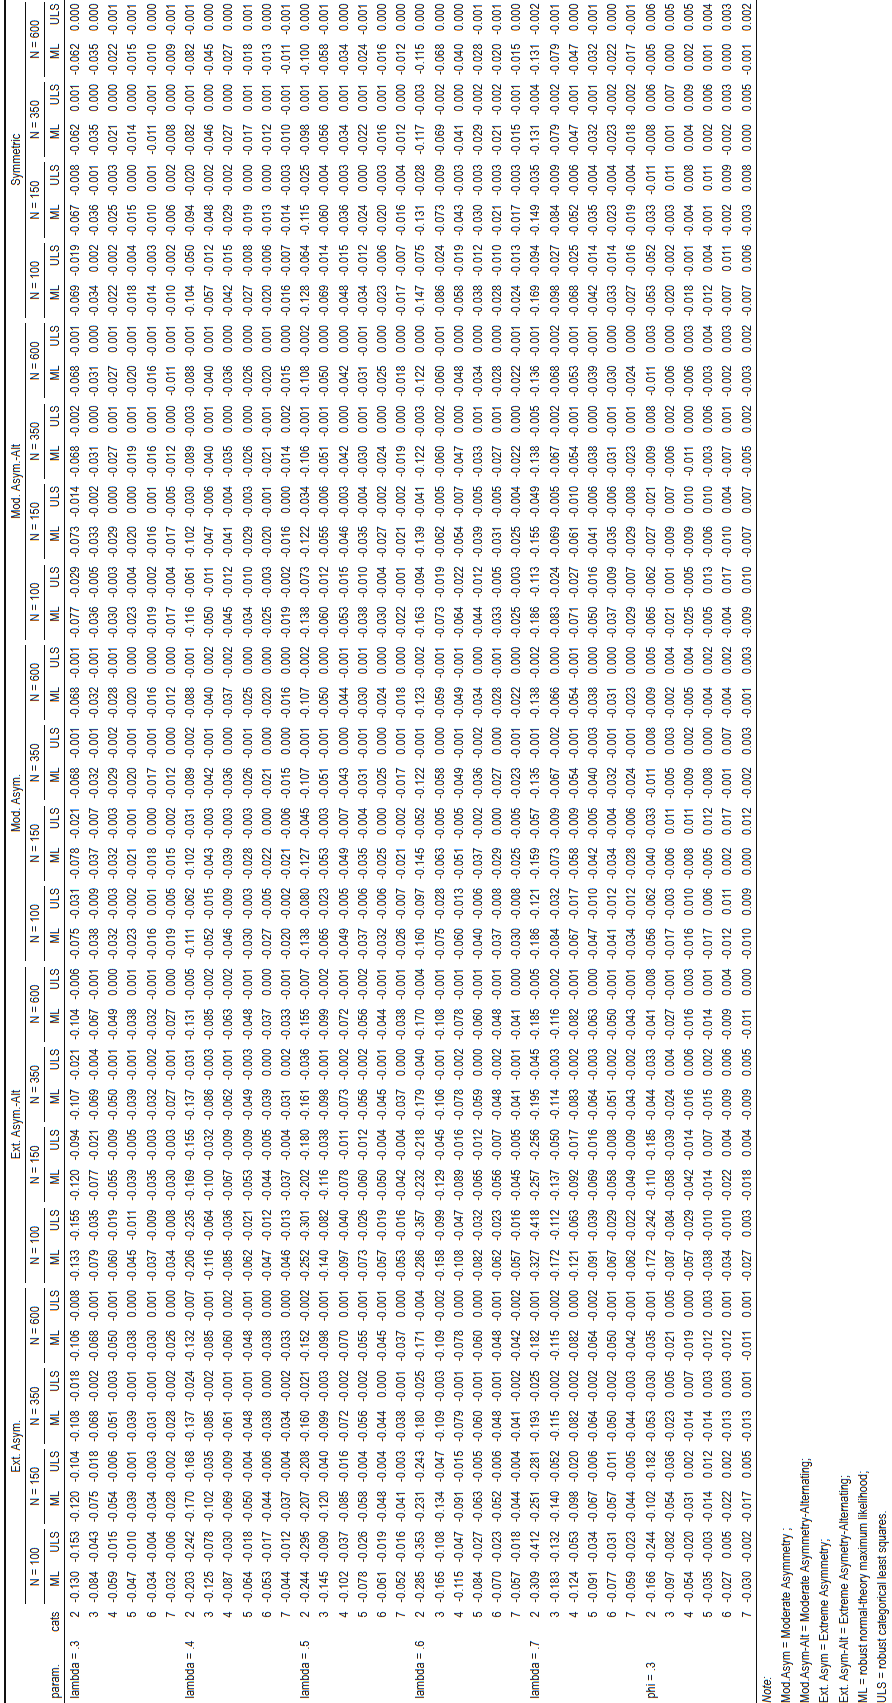
\includegraphics[width=325pt]{./figures/tabA8}

\subsubsection{Parameter Bias, Model2, Underlying Distribution = Skew 2, Kurtosis 7 (A9)}

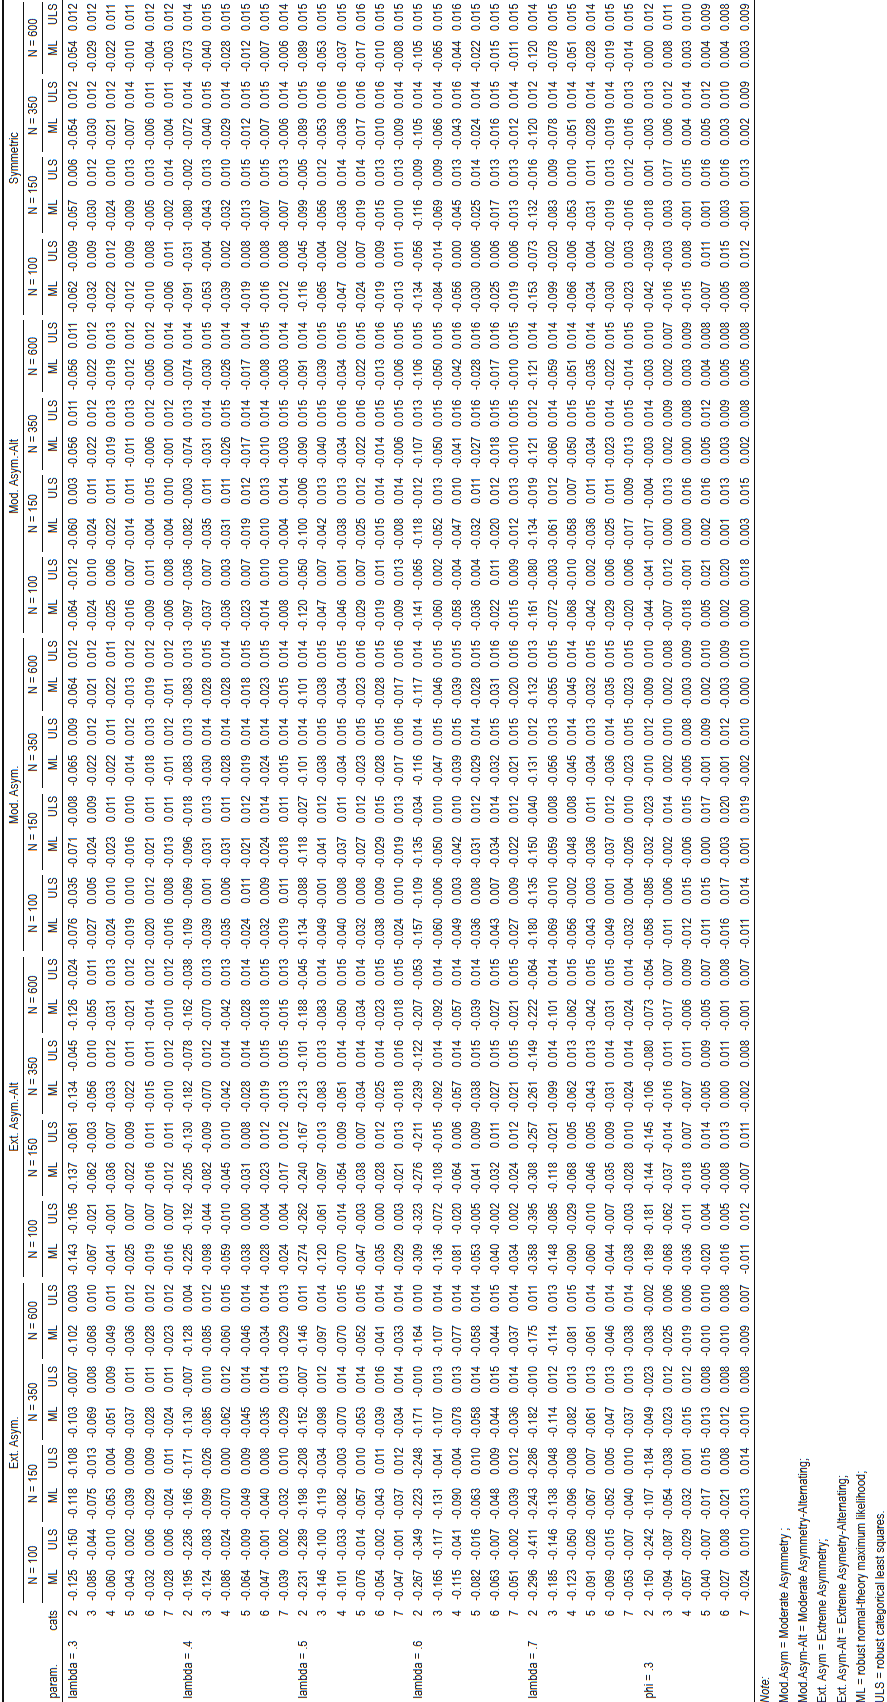
\includegraphics[width=325pt]{./figures/tabA9}

\subsubsection{Efficiency, Model- 1, Underlying Distribution = Normal (A10)}

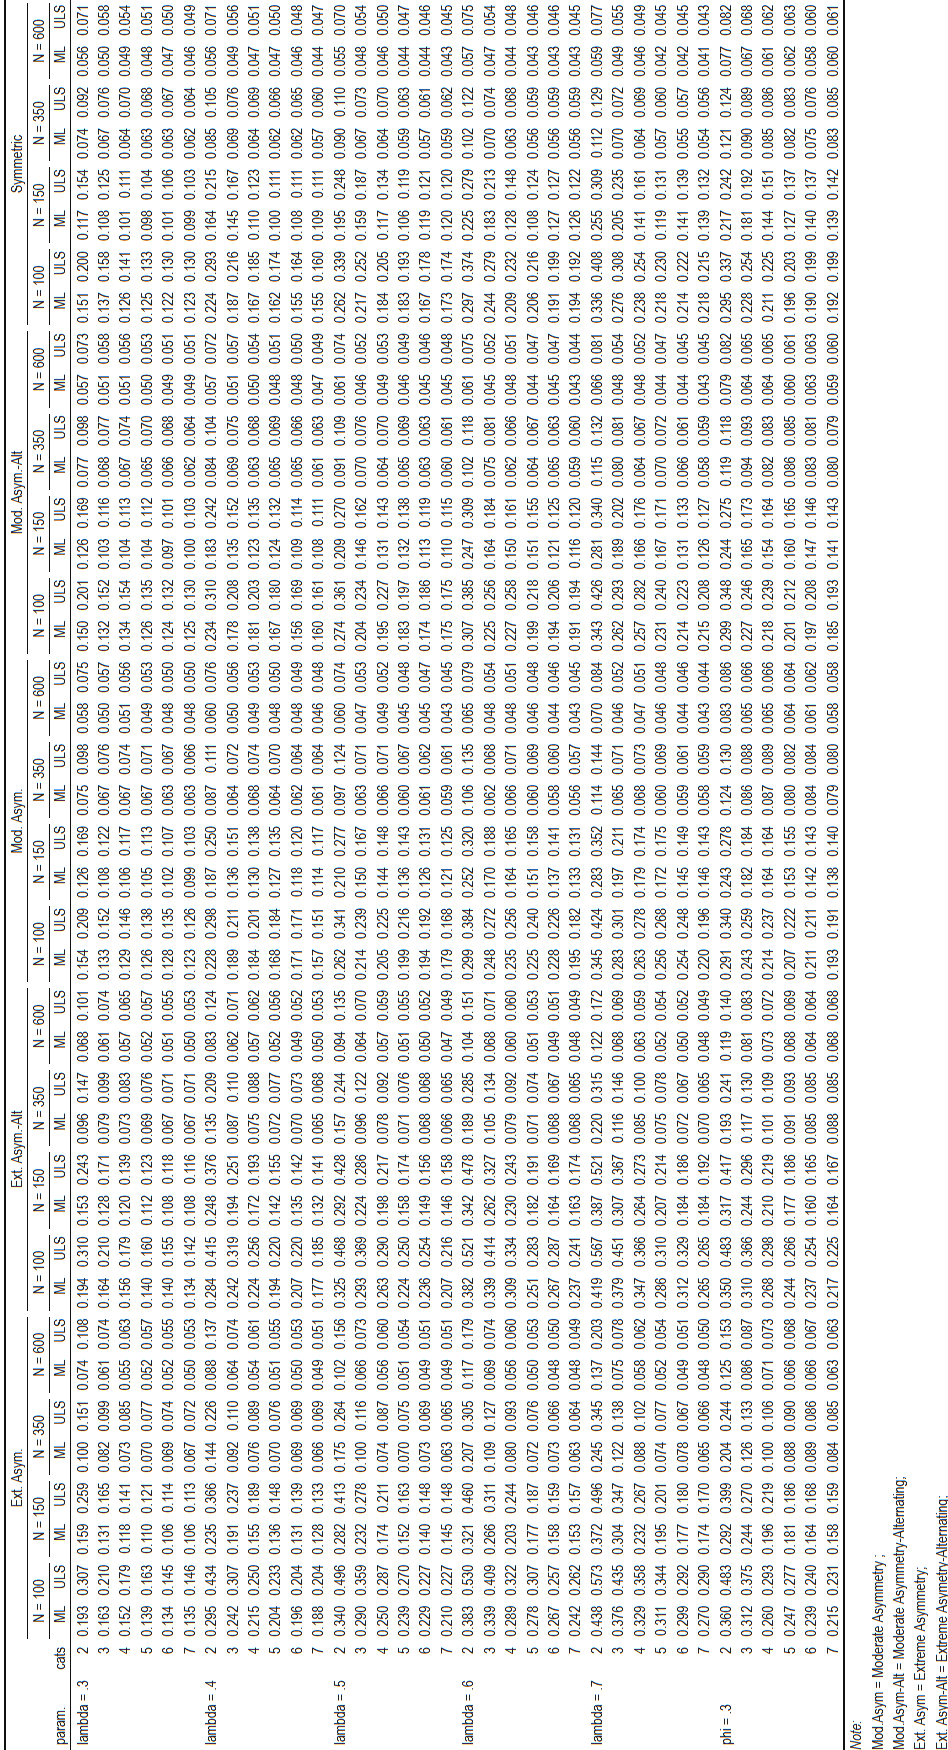
\includegraphics[width=325pt]{./figures/tabA10}

\subsubsection{Efficiency, Model- 1, Underlying Distribution = Skew 2, Kurtosis 7 (A11)}

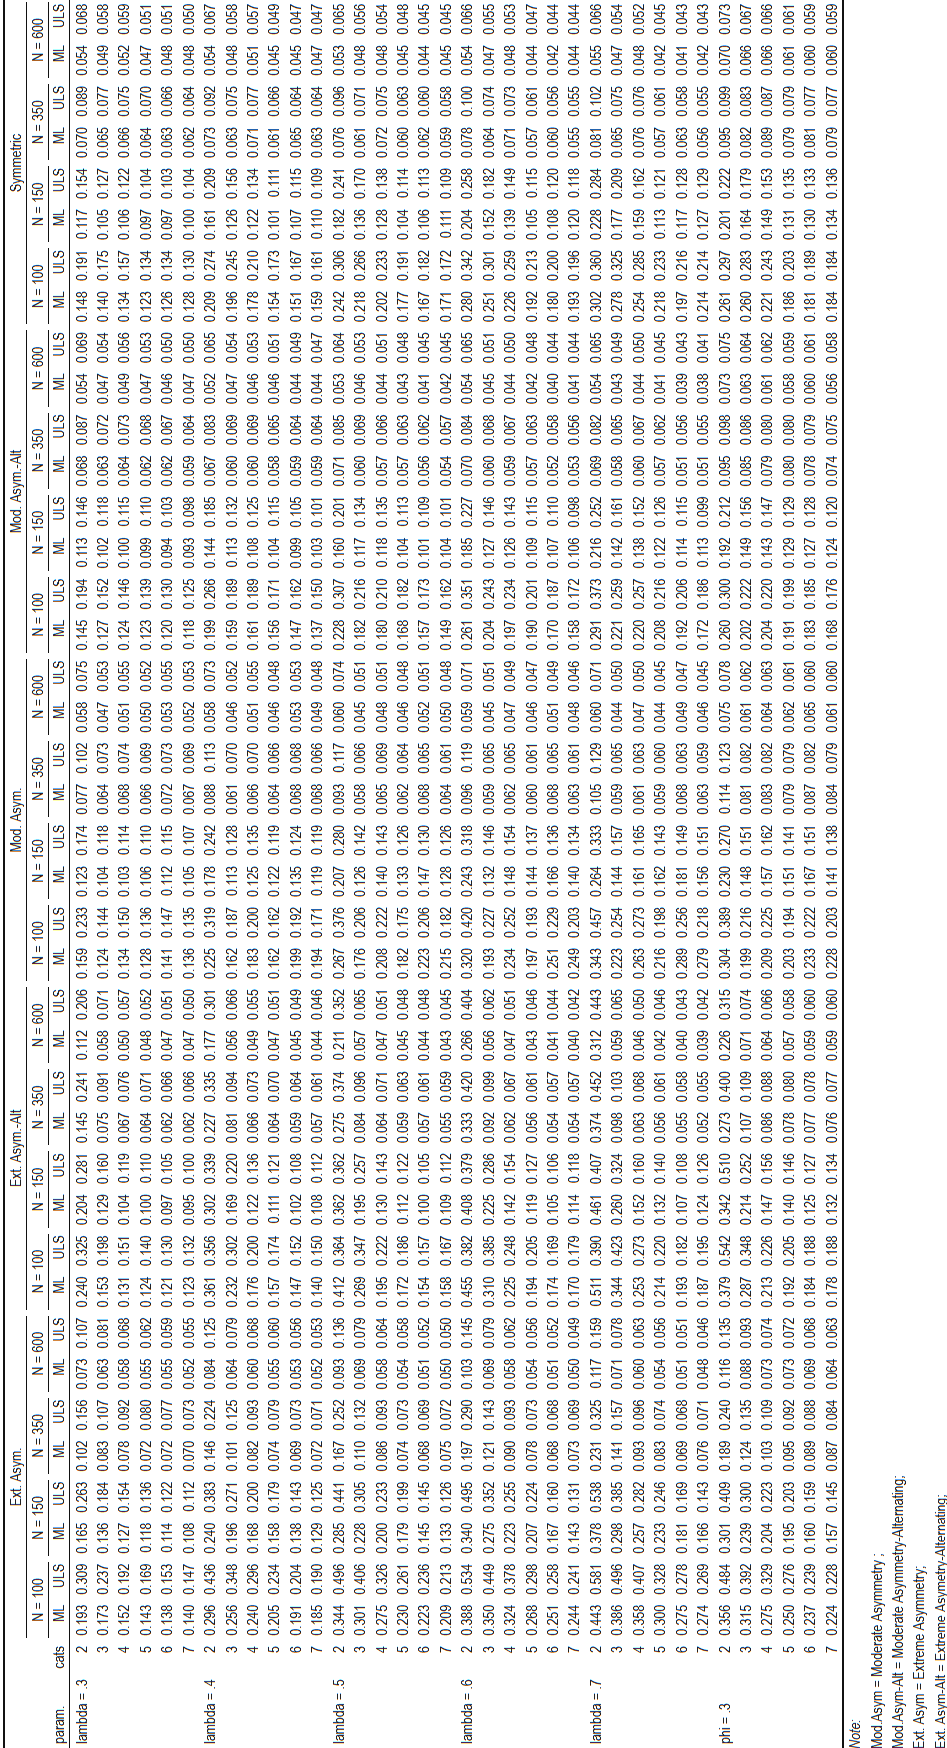
\includegraphics[width=325pt]{./figures/tabA11}

\subsubsection{Efficiency, Model- 2, Underlying Distribution = Normal (A12)}

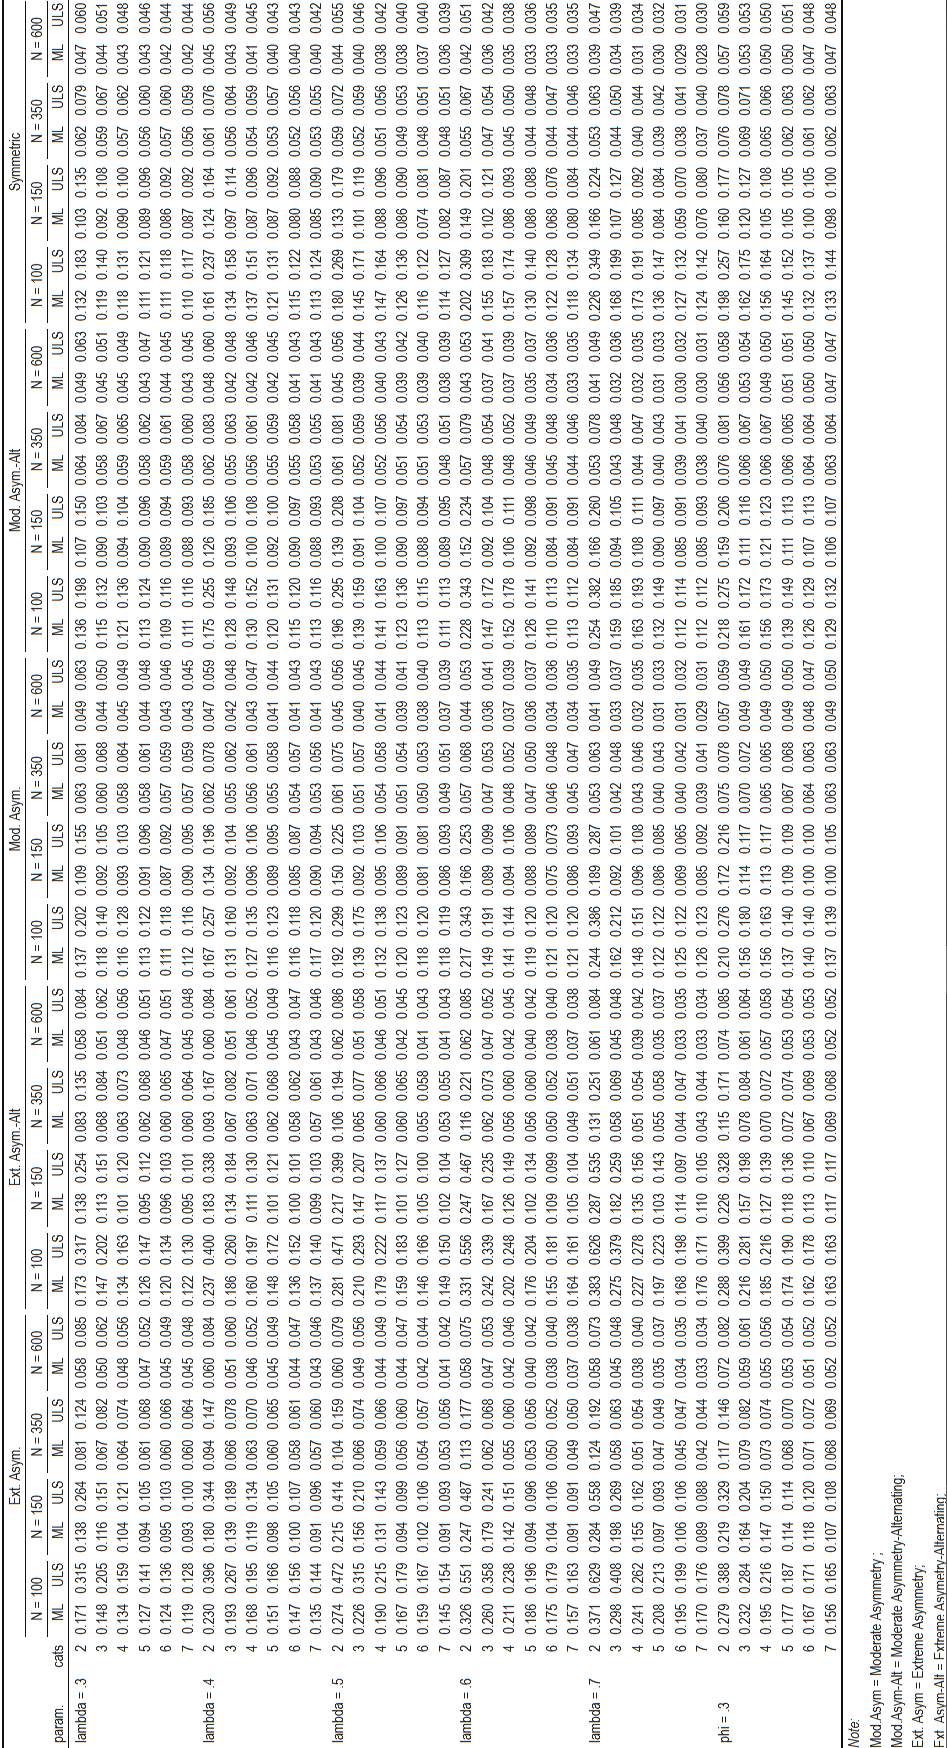
\includegraphics[width=325pt]{./figures/tabA12}

\subsubsection{Efficiency, Model- 2, Underlying Distribution = Skew 2, Kurtosis 7 (A13)}

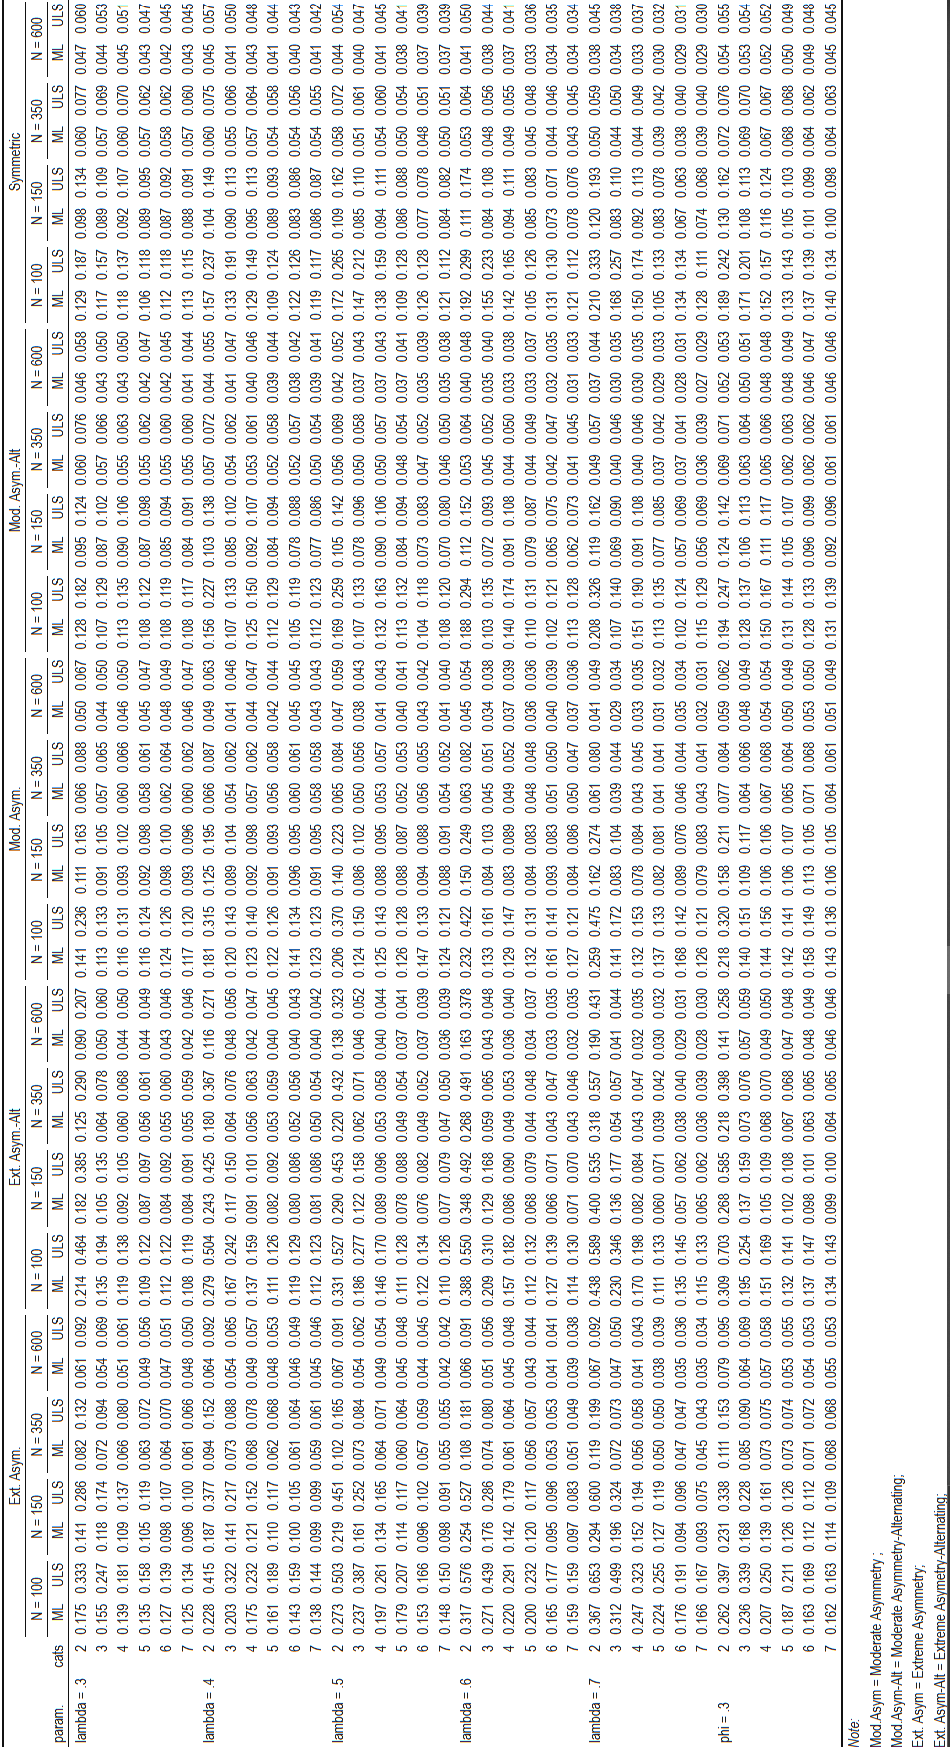
\includegraphics[width=325pt]{./figures/tabA13}

\FloatBarrier
\section{Discussion}

\subsection{Replicability}

Due to the high amount of details in the original publication and the
corresponding supplemental materials the replication was straight
forward. The largest amount of time was spent ensuring that the methods
used for data generation and analysis did indeed correspond to what was
used in the original study. This is, however, in no way the fault of the
authors but rather due to limited documentation of the R packages used
for replication. On the contrary, the detailed description of the
implementation allowed for a close correspondence of methodology which
would have otherwise been left to guesswork.

A feature that deserves special praise with regards to facilitating
replicability is the high amount of documentation that the authors
dedicated to the generation of the simulated data as well as the
descriptives of the same. The ability to closely monitor the data
generation process and compare features of the simulated data to the
original study instilled a great deal of confidence in the replicators
and ensured that any potential deviations of results could not be
attributed to faulty interpretation and implementation of the data
generating mechanism.

Another feature that increased reproducibility was the structure of the
manuscript. The very first element of the method section was an overview
of the simulation factors. Readability was increased by listing each
factor as a separate bullet point. Subsequent sections detailed the
implementation of each simulation factor. A separate subheading for each
simulation factor made it easy to locate relevant information.

The large number of result tables presented in the supplemental material
is another exemplary reporting practice worth highlighting. While the
comparison of hundreds of table cells is not an easy endeavor and the
general interest in these tables likely limited it protects the authors
against any allegations of selective reporting and makes the assessment
of replicability possible.

A similar structure could be found for the performance measures which
were discussed in separate subsections separated by corresponding
headings. While very readable as is, we would have however preferred the
performance measures to be elaborated on as part of the method section
instead of the result section.

The introduction section included the presentation and discussion of
several closely related methods as well as findings from previous
studies investigating the same. Due to the large amount of information
surrounding highly similar methods and their implementation it took us
several readings of the introduction to feel confident about having
identified the version actually implemented in the study at hand. A
clearer separation of the implemented methods (e.g.~in a box) would have
facilitated isolating the relevant implementation details.

Finally, a major factor facilitating the reproduction process was the
availability of specialized SEM software in the R programming
environment. As R is frequently used for simulation studies
investigating SEM methodology we were able to build upon a code base
that was designed for this very purpose. While such specialized software
has the potential of huge time savings on the coding end and
additionally is likely to minimize coding errors on the part of the
replicator it consumes a significant amount of time to familiarize
oneself with the exact parameters underlying the tools. The
inexperienced user is at the mercy of the package documentation and the
occasional peek under the hood of a given function. Having a code base
from related simulation studies available would increase confidence in
using such tools and avoid some trial and error while familiarizing
oneself with the functionalities.

\subsection{Replicator degrees of freedom}

We judge the replicator degrees of freedom in this replication to be
very minimal. The only area for clarification regards error handling
where simply stating whether case or list wise deletion was applied
would have been helpful.

\subsection{Equivalence of results}

Although our replicated results do not perfectly align with the original
study's findings, the conclusions drawn by the authors largely mirror
our own. Due to detailed descriptions of error frequency, we were able
to detect that any scenarios with large discrepancies from the original
study corresponded to scenarios with high numbers of errors.

Figure 1 and 2 as well as Table 1 suggest that our implementation of the
data generating mechanism produced data sets resembling those of the
original study. Any discrepancies in results are thus likely due to
differences in model estimation. Our results indicate poor performance
of both estimators at low sample size and low numbers of categories.
Given the large number of errors (also encountered in the original
study) it would have been advisable to report Monte Carlo errors to
allow a more nuanced comparison of the magnitude of discrepancies.

\section{Contributions}

Authors made the following contributions according to the CRediT
framework \url{https://casrai.org/credit/}

Anna Lohmann:

\begin{itemize}
\tightlist
\item
  Data Curation\\
\item
  Formal Analysis (lead)\\
\item
  Investigation\\
\item
  Software\\
\item
  Visualization
\item
  Writing - Original Draft Preparation\\
\item
  Writing - Review \& Editing
\end{itemize}

Arjan Huizing:

\begin{itemize}
\tightlist
\item
  Formal Analysis (supporting)\\
\item
  Investigation\\
\item
  Software
\item
  Validation\\
\item
  Writing - Review \& Editing
\end{itemize}

\newpage

\section*{References}
\begingroup
\hphantom{x}
\setlength{\parindent}{-0.5in}
\setlength{\leftskip}{0.5in}

\hypertarget{refs}{}
\begin{CSLReferences}{1}{0}
\leavevmode\vadjust pre{\hypertarget{ref-rougier_sustainable_2017-1}{}}%
Rougier, Nicolas P., Konrad Hinsen, Frédéric Alexandre, Thomas Arildsen,
Lorena A. Barba, Fabien C. Y. Benureau, C. Titus Brown, et al. 2017.
{``Sustainable Computational Science: The {ReScience} Initiative.''}
\emph{PeerJ Computer Science} 3 (December): e142.
\url{https://doi.org/10.7717/peerj-cs.142}.

\end{CSLReferences}

\FloatBarrier
\endgroup
\newpage

\section*{Appendix}

\subsection{Code organization}

The code and the files associated are organized in the form of a
research compendium which can be found in the following git repository
\texttt{https://github.com/replisims/rhemtulla-2012}

\begin{verbatim}
## ../..
## +-- analysis
## +-- data
## +-- data-raw
## +-- DESCRIPTION
## +-- dump
## +-- inst
## +-- man
## +-- NAMESPACE
## +-- R
## +-- results
## +-- rhemtulla-2012.Rproj
## +-- simfitALL.rds
## +-- simfitML.rds
## +-- simreps.rds
## +-- sim_fit_all_joined.rds
## +-- sim_fit_all_unnest.rds
## +-- sim_fit_all_unnest_alt.rds
## +-- sim_fit_all_unnest_no_out.rds
## +-- sim_fit_cov.rds
## +-- sim_fit_cov_no_out.rds
## +-- sim_powerML.rds
## +-- sim_powerULS.rds
## +-- sim_scenarios_id.rds
## \-- split_data
\end{verbatim}

\subsubsection*{Reproducibility Information}

This report was last updated on 2022-06-08 23:39:02. The simulation
replication was conducted using the following computational environment
and dependencies:

\FloatBarrier

\begin{verbatim}
## - Session info ---------------------------------------------------------------
##  setting  value
##  version  R version 4.1.3 (2022-03-10)
##  os       Windows 10 x64 (build 19043)
##  system   x86_64, mingw32
##  ui       RTerm
##  language (EN)
##  collate  English_United States.1252
##  ctype    English_United States.1252
##  tz       Europe/Berlin
##  date     2022-06-08
##  pandoc   2.17.1.1 @ C:/Program Files/RStudio/bin/quarto/bin/ (via rmarkdown)
## 
## - Packages -------------------------------------------------------------------
##  package        * version    date (UTC) lib source
##  assertthat       0.2.1      2019-03-21 [1] CRAN (R 4.1.2)
##  cachem           1.0.6      2021-08-19 [1] CRAN (R 4.1.2)
##  callr            3.7.0      2021-04-20 [1] CRAN (R 4.1.2)
##  cli              3.1.0      2021-10-27 [1] CRAN (R 4.1.2)
##  crayon           1.5.1      2022-03-26 [1] CRAN (R 4.1.3)
##  DBI              1.1.2      2021-12-20 [1] CRAN (R 4.1.2)
##  desc             1.4.1      2022-03-06 [1] CRAN (R 4.1.3)
##  devtools         2.4.3      2021-11-30 [1] CRAN (R 4.1.2)
##  digest           0.6.29     2021-12-01 [1] CRAN (R 4.1.2)
##  dplyr          * 1.0.8      2022-02-08 [1] CRAN (R 4.1.2)
##  ellipsis         0.3.2      2021-04-29 [1] CRAN (R 4.1.2)
##  evaluate         0.15       2022-02-18 [1] CRAN (R 4.1.3)
##  fansi            1.0.3      2022-03-24 [1] CRAN (R 4.1.3)
##  fastmap          1.1.0      2021-01-25 [1] CRAN (R 4.1.2)
##  fs               1.5.2      2021-12-08 [1] CRAN (R 4.1.2)
##  generics         0.1.2      2022-01-31 [1] CRAN (R 4.1.2)
##  glue             1.6.2      2022-02-24 [1] CRAN (R 4.1.2)
##  htmltools        0.5.2      2021-08-25 [1] CRAN (R 4.1.2)
##  knitr          * 1.38       2022-03-25 [1] CRAN (R 4.1.3)
##  lifecycle        1.0.1      2021-09-24 [1] CRAN (R 4.1.2)
##  magrittr         2.0.2      2022-01-26 [1] CRAN (R 4.1.2)
##  memoise          2.0.1      2021-11-26 [1] CRAN (R 4.1.2)
##  pillar           1.7.0      2022-02-01 [1] CRAN (R 4.1.2)
##  pkgbuild         1.3.1      2021-12-20 [1] CRAN (R 4.1.2)
##  pkgconfig        2.0.3      2019-09-22 [1] CRAN (R 4.1.2)
##  pkgload          1.2.4      2021-11-30 [1] CRAN (R 4.1.2)
##  prettyunits      1.1.1      2020-01-24 [1] CRAN (R 4.1.2)
##  processx         3.5.2      2021-04-30 [1] CRAN (R 4.1.2)
##  ps               1.6.0      2021-02-28 [1] CRAN (R 4.1.2)
##  purrr            0.3.4      2020-04-17 [1] CRAN (R 4.1.2)
##  R6               2.5.1      2021-08-19 [1] CRAN (R 4.1.2)
##  remotes          2.4.2      2021-11-30 [1] CRAN (R 4.1.2)
##  RepliSimReport   0.0.0.9000 2022-02-03 [1] Github (replisims/RepliSimReport@5f14003)
##  rlang            1.0.1      2022-02-03 [1] CRAN (R 4.1.2)
##  rmarkdown        2.13       2022-03-10 [1] CRAN (R 4.1.3)
##  rprojroot        2.0.2      2020-11-15 [1] CRAN (R 4.1.2)
##  rstudioapi       0.13       2020-11-12 [1] CRAN (R 4.1.2)
##  sessioninfo      1.2.2      2021-12-06 [1] CRAN (R 4.1.2)
##  stringi          1.7.6      2021-11-29 [1] CRAN (R 4.1.2)
##  stringr          1.4.0      2019-02-10 [1] CRAN (R 4.1.2)
##  testthat         3.1.1      2021-12-03 [1] CRAN (R 4.1.2)
##  tibble           3.1.6      2021-11-07 [1] CRAN (R 4.1.2)
##  tidyselect       1.1.2      2022-02-21 [1] CRAN (R 4.1.3)
##  usethis          2.1.5      2021-12-09 [1] CRAN (R 4.1.2)
##  utf8             1.2.2      2021-07-24 [1] CRAN (R 4.1.2)
##  vctrs            0.3.8      2021-04-29 [1] CRAN (R 4.1.3)
##  withr            2.5.0      2022-03-03 [1] CRAN (R 4.1.3)
##  xfun             0.30       2022-03-02 [1] CRAN (R 4.1.3)
##  xtable         * 1.8-4      2019-04-21 [1] CRAN (R 4.1.2)
##  yaml             2.3.5      2022-02-21 [1] CRAN (R 4.1.2)
## 
##  [1] C:/Users/alohmann/Documents/R/win-library/4.1
##  [2] C:/Program Files/R/R-4.1.3/library
## 
## ------------------------------------------------------------------------------
\end{verbatim}

The current Git commit details are:

\begin{verbatim}
## Local:    test C:/Users/alohmann/Dropbox (Personal)/anna/projects_new/replisims/replications/rhemtulla-2012
## Remote:   test @ origin (https://github.com/replisims/rhemtulla-2012.git)
## Head:     [1751d14] 2022-06-08: Finalize Report
\end{verbatim}


\end{document}
